\documentclass[specification,annotation,times]{itmo-student-thesis}
%% \documentclass[times]{itmo-student-thesis}

%% Опции пакета:
%% - specification - если есть, генерируется задание, иначе не генерируется
%% - annotation - если есть, генерируется аннотация, иначе не генерируется
%% - times - делает все шрифтом Times New Roman, собирается с помощью xelatex
%% - pscyr - делает все шрифтом Times New Roman, требует пакета pscyr.

%% Делает запятую в формулах более интеллектуальной, например:
%% $1,5x$ будет читаться как полтора икса, а не один запятая пять иксов.
%% Однако если написать $1, 5x$, то все будет как прежде.
\usepackage{icomma}

%% Один из пакетов, позволяющий делать таблицы на всю ширину текста.
\usepackage{tabularx}

%% Мульти-иллюстрации
\usepackage[caption=false,font=footnotesize]{subfig}

%% Данные пакеты необязательны к использованию в бакалаврских/магистерских
%% Они нужны для иллюстративных целей
%% Начало
\usepackage{tikz}
\usetikzlibrary{arrows}
%% Конец

%% Указываем файл с библиографией.
\addbibresource{master-thesis.bib}

%% Указываем путь к иллюстрациям
\graphicspath{{img/}{live_img/}}

%% Шорткаты
\DeclareMathOperator{\argmin}{argmin}
\DeclareMathOperator{\argmax}{argmax}

%% Теоремы/определения
\theoremstyle{definition}

\newtheorem{definition-ru}{Определение}

\begin{document}

\studygroup{M4239}
\title{Децентрализованный алгоритм управления конвейерной системой с использованием методов мультиагентного обучения с подкреплением}
\author{Мухутдинов Дмитрий Вадимович}{Мухутдинов Д.В.}
\supervisor{Фильченков Андрей Александрович}{Фильченков А.А.}{к.ф-м.н.}{кафедра КТ}
\publishyear{2019}
%% Дата выдачи задания. Можно не указывать, тогда надо будет заполнить от руки.
\startdate{01}{сентября}{2017}
%% Срок сдачи студентом работы. Можно не указывать, тогда надо будет заполнить от руки.
\finishdate{31}{мая}{2019}
%% Дата защиты. Можно не указывать, тогда надо будет заполнить от руки.
\defencedate{07}{июня}{2019}

\addconsultant{Вяткин В.В.}{проф., д.т.н.}

\secretary{Павлова О.Н.}

%% Задание
%%% Техническое задание и исходные данные к работе
\technicalspec{Требуется разработать децентрализованный алгоритм управления
  конвейерной системы для транспортировки багажа. Алгоритм должен позволять
  контроллерам конвейерной сети динамически изменять свое поведение в целях
  адаптации под изменившиеся условия работы, такие как поломка одного из
  конвейеров или изменение интенсивности потока багажа. Алгоритм должен
  обеспечивать своевременную доставку багажных единиц до пунктов назначения, в
  то же время минимизируя энергопотребление всей системы в целом.
}

%%% Содержание выпускной квалификационной работы (перечень подлежащих разработке вопросов)
\plannedcontents{Пояснительная записка должна содержать обзор существующих
  результатов в сфере управления конвейерными системами, а также в сферах,
  имеющих непосредственное отношение к предложенному алгоритму (таких как
  сетевая маршрутизация и обучение с подкреплением). Также записка должна
  содержать подробное изложение предложенного алгоритма и данные
  экспериментального сравнения его производительности с производительностью
  существующих методов управления конвейерной системой, проведенного с помощью
  виртуальной имитационной модели конвейерной сети.
}

%%% Исходные материалы и пособия 
\plannedsources{\begin{enumerate}
  \item Richard S. Sutton and Andrew G. Barto. Reinforcement Learning: An Introduction. The MIT Press, 2012
  \item Mnih et al. Human-level control through deep reinforcement learning. Nature, 518(7540):529–533, 2015.
\end{enumerate}}

%%% Цель исследования
\researchaim{
  Разработка децентрализованного алгоритма управления конвейерной системой,
  способного адаптироваться к гетерогенным изменениям в условиях работы.
}

%%% Задачи, решаемые в ВКР
\researchtargets{\begin{enumerate}
    \item разработка виртуальной имитационной модели конвейерной сети,
      позволяющей проводить сравнительный анализ алгоритмов управления;
    \item реализация ряда известных алгоритмов управления конвейерной сетью (а
      также маршрутизации) в рамках разработанной имитационной модели;
    \item разработка алгоритма, соответствующего поставленным требованиям;
    \item экспериментальное сравнение разработанного алгоритма с существующими
      по качеству работы.
\end{enumerate}}

%%% Использование современных пакетов компьютерных программ и технологий
\addadvancedsoftware{Язык программирования Python 3.6}{Гл.
  \ref{chapter-algorithm}, \ref{experiments}}
  %% ; приложение \ref{apx:simulators}}
\addadvancedsoftware{Библиотека для дискретно-событийного моделирования
  SimPy}{Гл. \ref{chapter-algorithm}, \ref{experiments}}
  %% приложение \ref{apx:simulators}}
\addadvancedsoftware{Библиотека для операций с графами NetworkX}{Гл.
  \ref{chapter-algorithm}, \ref{experiments}}
  %% приложение \ref{apx:simulators}}
\addadvancedsoftware{Математические пакеты NumPy и SciPy}{Гл.
  \ref{chapter-algorithm}, \ref{experiments}}
  %% приложение \ref{apx:simulators}}
\addadvancedsoftware{Библиотеки для машинного обучения scikit-learn и
  PyTorch}{Гл. \ref{chapter-algorithm}, \ref{experiments}}
  %% приложение \ref{apx:simulators}}
\addadvancedsoftware{Среда интерактивной разработки Jupyter Lab}{Гл.
  \ref{chapter-algorithm}, \ref{experiments}}
  %% приложение \ref{apx:simulators}}
\addadvancedsoftware{Библиотеки Matplotlib, Seaborn и Pandas для обработки и
  визуализации данных}{Гл. \ref{chapter-algorithm}, \ref{experiments}}
  %% приложение \ref{apx:simulators}}

%%% Краткая характеристика полученных результатов 
\researchsummary{
  Разработан алгоритм управления конвейерной системой на основе глубокого
  мультиагентного обучения с подкреплением. В ходе экспериментального
  исследования было установлено, что разработанный алгоритм превосходит
  существующие по качеству работы и способен адаптироваться к изменениям во
  внешней среде.
}

%%% Гранты, полученные при выполнении работы 
\researchfunding{
  Государственное задание № 2.8866.2017/БЧ <<Технология разработки программного
  обеспечения систем управления ответственными объектами на основе глубокого
  обучения и конечных автоматов>>
}

%%% Наличие публикаций и выступлений на конференциях по теме выпускной работы
\researchpublications{
\begin{refsection}
\nocite{mukhutdinov2019multi}
\nocite{mukhutdinov2019kmu}
\printannobibliography
\end{refsection}
}

%% Эта команда генерирует титульный лист и аннотацию.
\maketitle{Магистр}

%% Оглавление
\tableofcontents

%% Макрос для введения. Совместим со старым стилевиком.
\startprefacepage

Конвейерные системы широко применяются для автоматизированной транспортировки
объектов и материалов. Они являются неотъемлемой частью комплексов промышленного
оборудования, пунктов сортировки грузов, багажных систем в аэропортах и т. д..
Оптимизация работы таких системы имеет высокую практическую и экономическую
значимость, что мотивирует поиск эффективных методов управления конвейерными
системами.

Для управления большинством современных конвейерных систем применяются
централизованные статические стратегии управления, специально разрабатываемые
под конкретную систему одновременно с проектированием ее физической топологии в
целях решения задач конкретного предприятия \cite{de1994baggage}. Преимуществами
такого подхода являются высокая производительность работы и предсказуемость
поведения системы. Недостатками такого подхода являются высокая стоимость и
долгие сроки разработки кастомизированной стратегии управления, неспособность
системы адаптироваться к изменениям во внешний условиях, не учтенных во время
проектирования (таким как неожиданный отказ отдельных элементов системы), а
также наличие централизованного контроллера как критической точки отказа.

В связи с обозначенными недостатками использования кастомизированных стратегий
управления существует интерес к разработке обобщенных систематических подходов к
управлению конвейерными системами. Наиболее популярным подходом из используемых
является управление с прогнозируемыми моделями (\textit{англ.} model predictive
control, MPC) \cite{qin2003survey}. Управление с прогнозируемыми моделями
изначально разрабатывалось для задач химической промышленности и
нефтепереработки \cite{eaton1992model}, и на данный момент широко используется в
этих сферах. В последние несколько лет повысился интерес к применению данного
подхода к управлению другими типами киберфизических систем, в том числе
промышленными конвейерными линиями \cite{cataldo2016dynamic, luo2015energy} и
системами распределения багажа на основе рельсовых тележек (\textit{англ.}
destination coded vehicles, DCVs) \cite{tarau2010model, zeinaly2015integrated}.
Существующие алгоритмы на основе управления с прогнозируемыми моделями
обобщаются на различные конкретные конфигурации физических систем, но все еще
предусматривают наличие централизованного контроллера. Кроме того, модификация
существующего алгоритма управления (например, добавления учета энергопотребления
системы) во многих случаях является нетривиальной задачей, так как
оптимизируемая функция во фреймворке MPC должна выражаться как задача линейного
(\textit{англ.} linear programming, LP) или квадратичного программирования
(\textit{англ.} quadratic programming, QP). В связи с этим существует интерес к
разработке иных, децентрализованных подходов к управлению конвейерными сетями,
требующих менее строгих ограничений к характеру решаемой задачи.

При рассмотрении штучных конвейеров, перемещающих отдельные объекты, как в
случае систем для перемещения багажа в аэропортах, задачу управления конвейерной
системой можно декомпозировать на несколько подзадач, основными из которых являются задачи
маршрутизации объектов и предотвращения их столкновения.
Первая из этих подзадач по большей части сводится к задаче пакетной маршрутизации
(\textit{англ.} packet routing). Задача пакетной маршрутизации --- это задача
поиска пути наименьшей стоимости в графе из текущей вершины $n$ в вершину
назначения $d$. В контексте конвейерных систем топология конвейерной сети может
быть представлена в виде ориентированного графа, а перемещаемые по конвейерам
объекты могут быть абстрагированы как <<пакеты>>. 

Задача пакетной маршрутизации впервые обрела актуальность с появлением
компьютерных сетей. Первые алгоритмы сетевой маршрутизации появились в процессе
разработки сети ARPANet. Именно тогда были изобретены такие подходы к пакетной
маршрутизации, как дистанционно-векторный (\textit{англ.} distance-vector)
\cite{arpanet-orig} и состояния каналов связи (\textit{англ.} link-state)
\cite{link-state-arpanet}, которые и по сей день лежат в основе
таких стандартных и широко применяемых алгоритмов сетевой маршрутизации, как
Routing Information Protocol (RIP) \cite{rip-rfc} и Open Shortest Path First
(OSPF) \cite{ospf-rfc}. Преимуществами алгоритмов сетевой маршрутизации являются
обусловленные характером задачи децентрализованность, низкая требовательность к
вычислительным ресурсам и устойчивость к отказам маршрутизаторов и обрывам
соединений. В работе \cite{vyatkin-controllers} было продемонстрировано, что
простой дистанционно-векторный алгоритм маршрутизации может быть напрямую
применен к задаче управления конвейерной системой для транспортировки багажа,
что позволяет достигнуть устойчивости системы к отказам отдельных конвейеров.
Однако, в силу своей простоты, дистанционно-векторный алгоритм решает
исключительно задачу направления перемещаемых объектов вдоль кратчайших путей в
конвейерной сети, что ограничивает его применимость в тех случаях, когда
необходимо учитывать дополнительные критерии оптимизации (такие как
энергопотребление системы).

Cуществуют и другие подходы к решению задачи пакетной маршрутизации. Одним из
таких подходов является подход на основе идеи обучения с подкреплением
(\textit{англ.} reinforcement learing, RL). Первым таким алгоритмом стал алгоритм
Q-routing \cite{q-routing-orig}, основанный на методе Q-learning
\cite{q-learning-orig}. Этот алгоритм, как и его модификации
\cite{predictive-q-routing, dual-q-routing}, благодаря обучению с подкреплением
оказался способен лучше адаптироваться к изменениям в интенсивности сетевого
трафика, чем алгоритмы, основанные на вычислении кратчайшего пути. Но из-за
использования большого количества служебных сообщений, использующих те же каналы
передачи данных, что и целевые пакеты, применение таких алгоритмов в реальных
компьютерных сетях ограничено.

В контексте конвейерных сетей, однако, целевые <<пакеты>> являются физическими
объектами (например, чемоданами), перемещаемыми по конвейерной ленте, в то время
как служебные сообщения передаются по проводным соединениям между контроллерами.
Таким образом, время распространения служебных сообщений по системе пренебрежимо
мало по сравнению с временем перемещения целевых объектов, что нивелирует
озвученный недостаток алгоритмов маршрутизации, основанных на обучении с
подкреплением.

В данной работе будет предложено несколько модификаций гибридного децентрализованного
алгоритма управления конвейерной системой, основанного на методе Q-routing, но
использующего нейронную сеть в качестве обучающегося агента. Для демонстрации
способности работы алгоритма в различных постановках задачи маршрутизации он
будет исследован как в имитационной модели конвейерной системы, так и в
имитационной модели абстрактной компьютерной сети.

В главе 1 будет рассмотрена сама задача управления штучной конвейерной системой.
Она будет разбита на подзадачи, такие как задача маршрутизации, задача
избежания столкновений и задача оптимизации энергопотребления. Для каждой из
этих задач будут рассмотрены известные подходы к их решению, включая подходы
из смежных областей, таких как сетевая маршрутизация и управление другими типами
киберфизических систем. Также будет сформулирована обобщенная постановка
задачи маршрутизации в терминах мультиагентного обучения с подкреплением, к
которой будет сведена задача управления конвейерной системой. Будут рассмотрены
существующие алгоритмы маршрутизации, их сильные и слабые стороны. Также будут
рассмотрены существующие методы обучения нейронных сетей с подкреплением, в том
числе в мультиагентном случае.

В главе 2 будет рассмотрен предложенный алгоритм и его модификации и обоснованы
решения, принятые в ходе его разработки.

В главе 3 будут приведены экспериментальные результаты работы алгоритма для
задач пакетной маршрутизации в моделях компьютерной сети и управления системой багажных
конвейеров. Также будет проведено экспериментальное сравнение алгоритма с
существующими алгоритмами маршрутизации и управления конвейерной системой.

%% Начало содержательной части.
\chapter{Обзор предметной области}

%% Так помечается начало обзора.
\startrelatedwork

\section{Задача управления конвейерной системой}\label{problem-statement}

Конвейерные системы имеют широкий спектр применения во многих различных областях
человеческой деятельности. Соответственно, существует множество различных видов
конвейеров и конвейерных систем. С инженерной точки зрения конвейерные системы
можно различать по принципу действия и по конструктивным характеристикам
--- их можно подразделить на ленчатые, пластинчатые, тележные и прочие.
Также конвееры различают по назначению, то есть по типу перемещаемых грузов и по
сфере применения.

С точки зрения математического моделирования конвейерной системы наиболее
осмысленно разделять конвейеры на два крупных множества -- для
перемещения штучных грузов и для перемещения насыпных (или кусковых) грузов.
В первом случае перемещаемые по системе грузы можно моделировать как множество
дискретных объектов, где каждый объект имеет свою определенную позицию, во
втором случае так делать нельзя. Также эти типы конвейеров решают разные задачи,
и соответсвенно, требуют различных подходов к оптимизации своей работы.

В данной работе будет рассмотрена задача управления конвейерной системой для
перемещения штучных грузов. В качестве конкретной рассматриваемой задачи выбрана
задача управления системой ленчатых (пластинчатых) конвейеров для
транспортировки багажа в аэропорту. Для проведения экспериментов 
была разработана имитационная модель конвейерной системы, описанная в Приложении
\ref{apx:simulators}.

При перемещении штучных грузов с помощью конвейерной системы очевидным критерием
оптимизации является скорость доставки груза до точки назначения. Для систем с
нелинейной топологией (какими, например, являются системы для транспортировки
багажа), кроме того, необходимо решать задачу избежания столкновений между
перемещаемыми объектами, и, более того, эта задача является приоритетной.
И для всех без исключения конвейерных систем, включая и системы для перемещения
насыпных грузов, актуальна задача оптимизации энергопотребления.

Далее мы рассмотрим эти три подзадачи и подходы к их решению по отдельности.

\subsection{Маршрутизация}\label{overview:routing}

Задача оптимизации скорости доставки груза до точки назначения с помощью
конвейерной системы по большей части сводится к задаче маршрутизации. В общем
случае, задача маршрутизации --- это задача поиска множества путей наименьшей
стоимости $P = \{(p^i, p_1^i, ... , p_k^i, d^i)\}_{i=0}^N$ в графе $G = (V, E)$ при
заданном множестве пар точек входа и точек назначения
$Q = \{(p^i, d^i)\}_{i=0}^N$ и некоторых заданных ограничениях на пути. Как
правило, за стоимость пути берется время его прохождения некоторым объектом,
находящемся в заданной точке входа --- например, время доставки пакета по адресу
в компьютерных сетях.

Большинство исследований, посвященных маршрутизации, посвящены исследованию
маршрутизации именно в компьютерных сетях, что неудивительно, учитывая ее
колоссальную практическую значимость. Наиболее важные в рамках данной работы
алгоритмы сетевой маршрутизации будут рассмотрены в разделе
\ref{overview:networks}. Сейчас мы рассмотрим существующие подходы к
маршрутизации в конвейерных системах, в особенности --- в системах
транспортировки багажа.

\subsubsection{Маршрутизация для насыпных конвейеров}\label{overview:japans}

В конвейерных системах для перемещения насыпных грузов задача маршрутизации
возникает, например, в тех случаях, когда нужно сортировать по разным точкам
назначения несколько типов разных материалов, поступающих из одного источника.
Такая задача часто возникает в рамках работы промышленных предприятий, например,
металлургических заводов.

Существуют методы оптимального решения этой задачи, основанные на ее
представлении в виде задачи линейного программирования
\cite{ago2007simultaneous}. Эти методы предполагают, что все запросы за
некоторый временной интервал планирования $T$ заранее известны, и подразумевают
централизованный расчет стратегии работы для всей системы. К тому же, в силу
существенно различных специфик работы между насыпными и штучными конвейерами,
нельзя сходу применить эти методы к задаче маршрутизации в штучных конвейерных
системах.

\subsubsection{Маршрутизация для штучных конвейеров}

Задача маршрутизации в конвейерных системах для перемещения штучных грузов очень
похожа на задачу маршрутизации в компьютерных сетях, если представить
конвейерную сеть в виде направленного графа, где узлами графа являются точки
назначения (входы, выходы и какие-либо промежуточные точки на пути грузов), а
ребрами являются секции конвейеров между сочленениями. Так как методы
маршрутизации в компьютерных сетях хорошо изучены и развиваются очень давно,
имеет смысл применять их также и к конвейерным сетям.

Среди конвейерных систем, перемещающих штучные грузы, одними из наиболее
распространных являются системы для транспортировки багажа. Они предназначены
для доставки багажа со стоек регистрации, где его оставляют пассажиры, к
разгрузочным портам терминалов вылета, а также от терминалов прибытия к местам
выдачи багажа.

В современных крупных аэропортах, где багаж необходимо перемещать на большие
расстояния, системы для транспортировки багажа часто состоят не только из
конвейеров, но также и из автоматических рельсовых тележек (\textit{англ.}
destination coded vehicles, DCVs) \cite{fay2005decentralized, tarau2010model}.
В таких случаях конвейеры перемещают багаж только до тележек и обратно. Однако,
чисто конвейерные системы транспортировки дешевле и проще в установке, поэтому
они остаются востребованными, особенно для небольших аэропортов
\cite{vickers1998passenger}.

\begin{figure}[!h]
  \caption{Отклонитель отклоняет сумку на смежный конвейер}\label{diverter-pic}
  \centering
  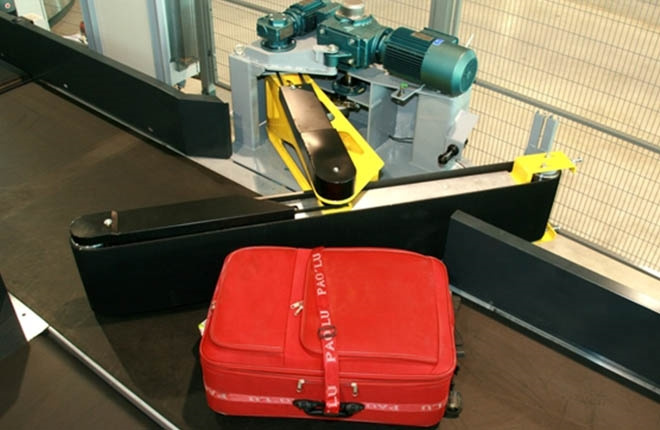
\includegraphics[width=0.6\textwidth]{diverter-photo}
\end{figure}

Ключевыми элементами конвейерной системы, помимо собственно конвейеров, являются
сканеры багажной бирки (\textit{англ.} scanner) и отклонители (\textit{англ.}
diverter) (рис. \ref{diverter-pic}). Последние играют роль агентов, выполняющих
маршрутизацию сумок в системе.

Отличительной чертой этих систем является невозможность применения к ним
статических методов оптимального контроля наподобие метода маршрутизации для
насыпных конвейеров, описанного в разделе \ref{overview:japans}. Это связано с
тем, что все запросы маршрутизации за некоторый период планирования $T$ не могут
быть известны заранее, так как
пассажиры регистрируют багаж на разные рейсы в случайном порядке, и информация о
наличии конкретной сумки появляется в системе только после прохождения сумкой
сканера \cite{hallenborg2007decentralized, de1994baggage}. Таким образом,
стратегия маршрутизации должна быть рассчитана для каждой новой сумки в
отдельности.

В существующих конвейерных системах по большей части применяется статический
подход к маршрутизации, когда для каждой новой сумки весь маршрут до конечной
точки назначения рассчитывается в момент ее сканирования
\cite{johnstone2009status}.
В некоторых системах применяется более динамический подход, аналогичный
маршрутизации в конвейерных сетях, когда кратчайший маршрут до точки назначения
рассчитывается при приближении сумки к очередному отклонителю (\textit{англ.}
diverter) \cite{hallenborg2007decentralized}. Однако, в обоих случаях стоимость
пути рассчитывается только с учетом длин конвейеров, например, с помощью
алгоритма Дейкстры. Второй подход в этом случае имеет больше смысла, чем первый,
только тогда, когда сумка может быть доставлена в любую из нескольких точек
назначения (например, в случае, если сумка должна быть доставлена к одному из
множества рентгеновских сканеров для проверки службой безопасности), и когда в
ходе работы системы какие-либо из этих точек могут стать недоступны (например,
когда выбранный ранее сканер занят другой сумкой).

В большинстве случаев, в системах для транспортировки багажа контроллеры
отклонителей на сочленениях не производят расчет стратегии, а только посылают
сообщения об обнаружении подъезжающей сумки центральному логическому узлу,
который, в свою очередь, посылает обратно сообщение с действием, которое
требуется совершить (сместить сумку/не смещать)
\cite{hallenborg2007decentralized, johnstone2009status}. Это еще одно
существенное отличие от маршрутизации в компьютерных сетях, так как
централизованная маршрутизация в компьютерных сетях довольно редко имеет смысл
(как правило, только в особых случаях, имеющих отношение к
программно-определенным сетям (\textit{англ.} software-defined networks, SDNs))
\cite{mao2017routing, wang2018machine}.

Однако, централизованный подход к управлению всегда подразумевает наличие
центральной точки отказа для всей системы --- собственно логического
контроллера. Очевидно, что это нежелательное свойство для киберфизических
систем, поэтому децентрализованные подходы к управлению являются более
предпочтительными. В следующем подразделе мы подробно рассмотрим существующий
такой подход.

\subsubsection{Децентрализованная маршрутизация в системе транспортировки
  багажа}\label{vyatkin-method}

Децентрализованный метод управления конвейерной системой для транспортировки
багажа был предложен в работах \cite{black2009intelligent, vyatkin-controllers}.
В этих работах описана архитектура и логика контроллеров отдельных элементов
системы для транспортировки багажа (конвейеры, сканеры, отклонители и т. д.) а
также протокол их взаимодействия на основе стандарта IEC 61499 \cite{IEC61499}.
Предложенная в них архитектура обладает следующими свойствами:

\begin{figure}[!h]
  \caption{Схема децентрализованной архитектуры конвейера}\label{vyatkin-convs}
  \centering
  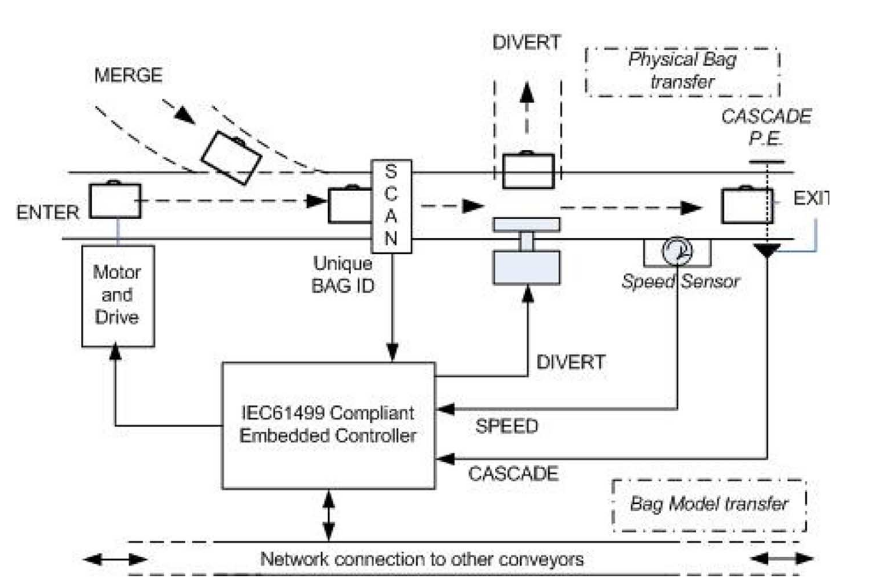
\includegraphics[width=\textwidth]{vyatkin-conveyors-illustration}
\end{figure}

\begin{itemize}
\item Каждый отдельный конвейер имеет свой логический контроллер
\item На конвейере в различных позициях могут находиться:
  \begin{itemize}
  \item сочленения с входящими конвейерами (\textit{англ.} mergers)
  \item сочленения с исходящими конвейерами, оборудованные отклонителями(\textit{англ.} diverters)
  \end{itemize} 
\item Перед каждым сочленением, как входящим, так и исходящим, установлен
  детектор, определяющий позицию сумки.
\item Сочлененные конвейеры соединены между собой коммуникационным интерфейсом и
  могут посылать друг другу сообщения.
\end{itemize}

На рисунке \ref{vyatkin-convs} представлена схема этой архитектуры.

Большая часть этих работ фокусируется на
технических деталях реализации логики контроллеров в рамках упомянутого
стандарта и изучением преимуществ его использования в сравнении с более старыми
архитектурными стандартами для программных контроллеров в киберфизических
системах (таких как IEC 61131-3 \cite{IEC61131}).

С точки зрения непосредственно
логики маршрутизации, в работах используется немного модифицированный
распределенный алгоритм Беллмана-Форда \cite{bellman-ford}, по сути, почти в
точности повторяющий логику дистанционно-векторных алгоритмов сетевой
маршрутизации (что будут рассмотрены более подробно в разделе
\ref{overview:networks:dv}). Работа \cite{vyatkin-controllers} отдельно
демонстрирует, что этот алгоритм способен адаптировать маршруты в случае поломок
отдельных конвейеров, точно так же, как дистанционно-векторный алгоритм в
компьютерных сетях способен адаптироваться к обрывам соединений. Это, вкупе с
отсутствием единой точки отказа, выгодно выделяет предложенный
децентрализованный подход на фоне общепринятых.

\subsection{Избежание столкновений}\label{overview:collisions}

Важнейшим ограничением на работу конвейерной системы любого предназначения
является недопущение столкновения перемещаемых объектов. Это ограничение
применимо и к конвейерным системам для насыпных грузов, в тех случаях, когда по
системе перемещаются грузы разного типа, смешение которых недопустимо.

Для систем, в которых для маршрутизации применяется расчет оптимальной стратегии
действий для заданного множества объектов в заданный промежуток времени, как в
работе \cite{ago2007simultaneous}, ограничение на запрет столкновений объектов
(или потоков материалов) можно выразить как одно из ограничений в задаче
линейного/квадратичного программирования (или же как один из членов
оптимизируемой функции с большим коэффициентом), чтобы выполненная глобальная
стратегия, будучи правильно исполненной, гарантированно не привела к столкновениям.

Однако, как уже было сказано, такой подход неприменим для решения задачи
управления системой транспортировки багажа. Вследствие этого в них, впрочем, как
и в других транспортных системах, применяются другие подходы.

Подход, основанный на взаимной координации скоростей соединяющихся конвейеров,
описан во многих источниках \cite{black2009intelligent, schafer2011material}.
Описания в них, в сущности, отличаются лишь глубиной и характером технических
деталей. Суть подхода во всех случаях одна и заключается во взаимной
синхронизации скоростей соединяющихся конвейеров при приближении объектов на них
к сочленению.

\begin{figure}[!h]
  \caption{Схема взаимодействия соединяющихся конвейеров при приближении сумки к
  сочленению}\label{collision-avoidance-1}
  \centering
  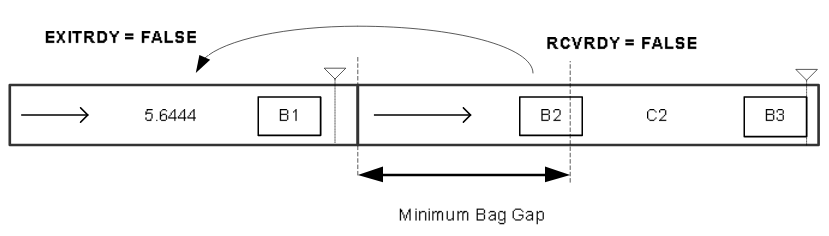
\includegraphics[width=\textwidth]{collision-avoidance-1}
\end{figure}

Для конкретики рассмотрим децентрализованный подход, описанный в
\cite{black2009intelligent}. Как было указано в предыдущем разделе, в нем
подразумевается, что каждый конвейер имеет собственный контроллер. Каждый
такой контроллер поддерживает модель положения сумок на соответствующем
конвейере. Такая модель поддерживается путем получения сигналов от детекторов,
стоящих в конце каждой секции конвейера, а также путем передачи сообщений о
входящих/исходящих сумках между соседними конвейерами.

В задачу системы входит поддержание установленного минимального зазора $D$ между
сумками. Если начало конвейера $C2$ находится, согласно текущей модели положения
сумок, на расстоянии меньшем $D$ от некоторой сумки, то въезд другой сумки на
начало конвейера запрещен. Конвейер сообщает об этом путем посылки специального
сигнала RCVRDY = FALSE предыдущему конвейеру $C1$, который, в свою очередь,
выставляет соответствущий флаг EXITRDY = FALSE. Аналогичным образом работают
сигналы MERGERDY и DIVERTRDY в случаях соединения конвейеров в сочленениях.

Если при приближении сумки в выходу или отклонителю соответствующий флаг
EXITRDY/DIVERTRDY имеет значение FALSE, то конвейер останавливается, не
допуская, чтобы сумка достигла конца текущей секции до тех пор, пока значение
флага не станет TRUE. Кроме того, конвейер выставляет все свой флаг RCVRDY и все
флаги MERGERDY, сообщая предыдущим конвейерам, что он останавливается и что на
него не следует перемещать сумки. При приближении сумок к такому конвейеру
предыдущие конвейеры будут также останавливаться, не допуская перемещение сумок
на него до тех пор, пока конвейер не возобновит работу. Таким образом
достигается, что между сумками, достигшими одного и того же сочленения,
соблюдается разумное расстояние, что исключает их столкновение.

В данной работе для избежания столкновений сумок будет использован именно этот
метод с небольшими модификациями в сочетании с разработанным алгоритмом маршрутизации.

\subsection{Оптимизация энергопотребления}\label{overview:energy}

Оптимизация энергопотребления конвейерных систем является крайне важной в
глобальном смысле задачей, так как на работу промышленных конвейерных систем
уходит до 6\% всей потребленной электроэнергии в мире \cite{halepoto2016design}.

Один из подходов к оптимизации энергопотребления --- усовершенствование
физического оборудования: разработка новых типов лент, смазок и натяжных колес
конвейеров в целях снижения побочных затрат энергии на трение и шум
\cite{staniak1996energy}. Еще один подход, не отрицающий первого --- снижение
энергопотребления путем контроля поведения конвейера.

Простейшим подходом к энергосбережению в конвейерных системах является
метод оптимального выключения (\textit{англ.} optimal switching control) ---
выключение конвейера в то время, когда он не выполняет полезной работы. Этот
подход, вообще говоря, применим не только к конвейерам, но и вообще к любому
автоматизированному оборудованию. Так, в работе
\cite{middelberg2009optimal} предложен метод оптимизации энергопотребления
разгрузочных конвейеров угольной шахты, основанный на методе оптимального
контроля, который определяет оптимальные временные промежутки для включения и
выключения конвейеров. Там же приведена формулировка этой задачи в обобщенной
форме как задачи минимизации функции

\begin{equation}\label{energy:opt-switching-J}
  J = \int_{t_0}^{t_1} \! \sum\limits_{i=1}^n P_i(t) u_i(t) p(t) \mathrm{d}t \,,
\end{equation}

где $[t_0, t_1]$ --- временной интервал планирования, $n$ --- количество
конвейеров, $P_i(t)$ --- энергопотребление $i$-го конвейера в момент времени
$t$, $p(t)$ --- функция, которая задает стоимость электроэнергии во время $t$
(дана как условие задачи), и

\begin{equation}\label{energy:opt-switching-u}
  u_i(t) = \begin{cases}
    1, & \text{if switched on}\\
    0, & \text{if switched off}
  \end{cases}
\end{equation}

--- контролируемая величина, определяющая, включен или нет конвейер $i$ в момент
времени $t$. Минимизация функции $J$ производится в соответствии с некоторыми
ограничениями вида

\begin{equation}\label{energy:opt-switching-g}
  g(u(t), t) \leq 0 \,,
\end{equation}

которые выражают операционные требования к системе (конвейеры должны
переместить груз, то есть они должны быть включены на момент поступления груза и
в то время, когда он находится на конвейере).

В случае системы транспортировки багажа, как уже было сказано, расписание
прибытия сумок не может быть известно заранее, что не позволяет использовать
данный подход к оптимизации энергопотребления. Однако, никто не запрещает
использовать простые эвристики, такие как остановка и выключение конвейера
спустя некоторое время после того, как на нем не осталось сумок
\cite{mukhutdinov2019multi}.

В случае, если включенный конвейер потребляет константное количество
электроэнергии за единицу времени, метод оптимального переключения является
наилучшим. Однако, на практике это не так.
На текущую энергоэффективность конвейера в каждый
конкретный момент времени влияет множество факторов: КПД двигателя, трение
ленты, масса перемещаемого груза, скорость движения и так далее. Зависимость
энергопотребления от этих параметров можно выразить с помощью математической
модели.

В целях проектирования и производства эффективного конвейерного
оборудования были разработаны стандартизированные модели расчета планируемого
энергопотребления, такие как ISO 5048 \cite{ISO5048}, DIN 22101 \cite{DIN22101}
и JIS B 9905 \cite{JISB8805}. Эти модели предназначены для конвейеров,
перемещающих насыпные грузы, и учитывают большое количество точных параметров
конструкции механизма, такие как масса вращающихся деталей, плотность
конвейерной ленты и так далее.

Как правило, ввиду своей сложности, данные модели не используются для
моделирования энергопотребления системы при решении задачи оптимизации. Для
оптимизации энергопотребления в работе \cite{zhang2011modeling} была предложена
приближенная аналитическая модель. Эта модель также предназначена для
конвейеров, перемещающих насыпные грузы, и выражает текущее энергопотребление
конвейера как:

\begin{equation}\label{energy:zhang-model}
  P(V, T) = \frac{1}{\eta} \left( \theta_1 VT^2 + \theta_2 V + \theta_3 \frac{T^2}{V}
  + \theta_4 T + \frac{V^2T}{3.6} \right) \,,
\end{equation}

где $V$ --- это текущая скорость конвейера, $T$ --- масса поступающего на вход
конвейера за единицу времени вещества, $\eta$ --- КПД системы, а $\theta_1$,
$\theta_2$, $\theta_3$ и $\theta_4$ --- коэффициенты, рассчитываемые из
постоянных характеристик конвейера, используемых в модели ISO 5048. 

В работе \cite{halepoto2016design} приводится простая обобщенная модель
энергопотребления конвейера для транспортировки штучных грузов:

\begin{equation}\label{energy:linear-model}
  P(V) = \frac{M_r(m_L)V}{\eta} \,,
\end{equation}

где $V$ --- это текущая скорость конвейера, $M_r$ --- это величина полного
сопротивления движению, зависящая от суммарной массы находящихся на конвейере
объектов $m_L$ и константных характеристик, таких как длина конвейера, его
ширина, и прочих.

Видно, что в этой модели энергопотребление линейно зависит от
скорости конвейера (если не учитывать тот факт, что от скорости конвейера
зависит скорость изменения $m_L$). В модели (\ref{energy:zhang-model}) тоже содержится
линейный член от $V$, что побуждает прийти к выводу, что в правдоподобных
моделях энергопотребления конвейера зависимость энергопотребления от скорости
похожа на линейную. Таким образом, если конвейер способен произвольно изменять
свою скорость, в целях снижения энергопотребления также имеет смысл регулировать
скорость конвейера, а не просто по возможности его выключать.

В разработанной в рамках данной работы имитационной модели конвейерной системы
для подсчета ``реальных'' затрат на электроэнергию используется модифицированная
под нужды штучных конвейеров модель (\ref{energy:zhang-model}).

%% \section{Методы оптимального контроля}

%% MPC \cite{luo2015energy}

%% \begin{definition-ru}
%%   \textbf Управление с прогнозируемыми моделями (\textit{англ.} model predictive
%%   control, MPC) --- это...
%% \end{definition-ru}

%% TBD

\section{Алгоритмы сетевой маршрутизации}\label{overview:networks}

Подавляющее большинство существующих алгоритмов маршрутизации разработаны именно
для применения в компьютерных сетях. Среди большого множества известных
алгоритмов маршрутизации в компьютерных сетях можно выделить два класса
наиболее широко распространенных алгоритмов --- дистанционно-векторные
(\textit{англ.} distance-vector) \cite{arpanet-orig} и состояния каналов связи
(\textit{англ.} link-state)
\cite{link-state-arpanet}. К каждому из этих классов относится множество различных
алгоритмов, различающихся техническими деталями, но работающих по одному
принципу. Далее мы рассмотрим только общие принципы работы алгоритмов из этих
классов, опуская детали реализации отдельных их представителей.

\subsubsection{Дистанционно-векторные алгоритмы}\label{overview:networks:dv}

%% \begin{figure}[!h]
%%   \caption{Иллюстрация работы distance-vector алгоритма}\label{rip-img}
%%   \centering
%%   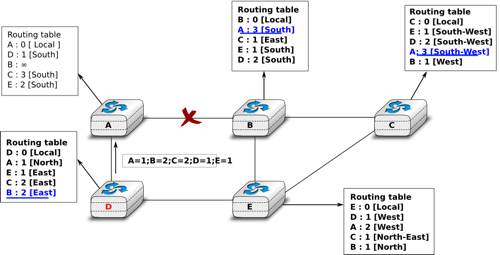
\includegraphics[scale=1.5]{dv-failure-2}
%% \end{figure}

\begin{algorithm}[!h]
\caption{Процесс обновления вектора кратчайших расстояний. $x$ -- текущий узел,
$y$ --- сосед, приславший собственный вектор расстояний $D_y$, $w$ --- вес ребра
  $(x, y)$, $V$ --- множество всех узлов в сети.}
\label{dv-pseudocode}
\begin{algorithmic}[1]
	\Procedure{UpdateDV}{$x$, $y$, $w$, $D_y$}
	  \For{$d \gets V$}
      \State $(l_x, n_x) \gets D_x(d)$
      \State $(l_y, n_y) \gets D_y(d)$
		  \If{$l_y + w < l_x$ \textbf{or} $n_x = y$}
				\State $D_x(d) \gets (l_y + w, n_y)$
			\EndIf
		\EndFor
	\EndProcedure
\end{algorithmic}
\end{algorithm}

В дистанционно-векторных алгоритмах каждый маршрутизатор поддерживает
\textit{вектор кратчайших расстояний} до всех остальных узлов в сети. Кроме
собственно кратчайших расстояний, в этом векторе содержатся метки первых соседей
текущего узла на соответствующих кратчайших путях. Расстояние до недостижимых
узлов полагается равным бесконечности, соответствующий сосед для таких узлов не
определен. Перенаправление пакета с узлом назначения $d$, таким образом,
осуществляется к соседу, хранящемуся для узла $d$ в векторе кратчайших
расстояний.

При обнаружении обрыва соединения (или, в общем случае, изменения веса смежного
соединения) маршрутизатор, обновив соответствующим образом собственный вектор
расстояний, рассылает его соседям, которые соответственно обновляют собственные
вектора (листинг \ref{dv-pseudocode}) и рассылают их далее.

Дистанционно-векторные алгоритмы просты в реализации и крайне нетребовательны к
памяти и вычислительным ресурсам, но медленно распространяют информацию об
изменениях по сети и сталкиваются с проблемами в при изменении топологии сети в
определенных случаях (проблема count-to-infinity). Алгоритмы из рассмотренного в
следующем подразделе класса избавлены от этих недостатков.

\subsubsection{Алгоритмы состояния канала связи}\label{overview:link-state}

\begin{algorithm}[!h]
\caption{Логика link-state маршрутизатора. В каждой процедуре, $x$ -- метка
  текущего узла, $G_x = (V_x, E_x)$ -- текущий граф сети, $W_x(u, v)$ -- вес ребра
  $(u, v)$.}
\label{ls-pseudocode}
\begin{algorithmic}[1]
  \Procedure{InitLS}{$x$, $N_x$}\Comment{$N_x$ -- список соседей вершины $x$}
    \State $V_x \gets \{x\}$
    \State $E_x \gets \emptyset$
    \For{$(y, w) \gets N_x$}
      \State $S_x(y) \gets 0$
    \EndFor
    \State \Call{UpdateLS}{$x$, $x$, 1, $N_x$}
  \EndProcedure
  \Statex
  \Procedure{AnnounceLS}{$x$}
    \State $N_x \gets \{(y, W_x(x, y)) | (x, y) \in E_x\}$
    \For{$(x, y) \gets E_x$} 
      \State \Call{UpdateLS}{$y$, $x$, $S(x)$, $N_x$}
    \EndFor
    \State $S_x(x) \gets S_x(x) + 1$
  \EndProcedure
  \Statex
	\Procedure{UpdateLS}{$x$, $y$, $s_y$, $N_y$}
    \If{$s_y > S_x(y)$}
      \For{$(z, w) \gets N_y$} \Comment{$w$ -- вес ребра до соседа}
        \State $V_x \gets V_x \cup \{z\}$
        \State $E_x \gets E_x \cup \{(y, z)\}$
        \State $W_x(y, z) \gets w$
      \EndFor
      \State $E_x \gets E_x \setminus \{(y, z) | z \notin \{z | (z, w) \in N_y \} \}$
      \State $S_x(y) \gets s_y$
      \For{$(x, z) \gets E_x$} 
        \State \Call{UpdateLS}{$z$, $y$, $s_y$, $N_y$}
      \EndFor
    \EndIf
	\EndProcedure
\end{algorithmic}
\end{algorithm}

В алгоритмах состояния канала связи каждый маршрутизатор поддерживает модель
всей сети в виде графа. При обрыве или восстановлении смежного ребра, а также при
изменении его веса маршрутизатор рассылает по сети обновленные состояния
собственных смежных ребер. Логика распространения информации по сети приведена в
листинге \ref{ls-pseudocode}.

Таким образом, при обработке очередного пакета маршрутизатор посылает в него
вдоль кратчайшего пути до узла назначения, который находится по текущей модели
графа, например, с помощью алгоритма Дейкстры \cite{dijkstra}. 

Алгоритмы из класса link-state обеспечивают более высокую скорость
распространения информации по сети и, соответственно, более быструю адаптацию
к обрывам и восстановлениям соединений. На текущий момент именно алгоритмы из
этого класса (например, OSPF \cite{ospf-rfc}) являются наиболее часто
используемыми в реальных компьютерных сетях. Однако, большинство таких
алгоритмов использует статические или редко обновляемые оценки весов соединений,
что приводит к плохой производительности в условиях высоконагруженного трафика
для некоторых топологий сетей.

\subsubsection{Q-routing}\label{q-routing-desc}

Алгоритм Q-routing \cite{q-routing-orig} является первым алгоритмом, в описании
которого задача маршрутизации интерпретируется как задача обучения с
подкреплением. Каждый маршрутизатор $x$ поддерживает таблицу $Q_x(d, y)$,
содержащую оценки стоимостей кратчайших путей до вершины $d$ через каждого из соседей
$y$. Пересылка пакета одному из соседей интерпретируется как \textit{действие},
за которое маршрутизатор получает \textit{вознаграждение} (равное времени,
потраченное пакетом на преодоление исходящего ребра) и оценку стоимости
дальнейшего пути от соседа (см. листинг \ref{qr-pseudocode}). 

\begin{algorithm}[!h]
\caption{Логика алгоритма Q-routing. $x$ -- метка текущего узла, $p$ -- ID пакета.}
\label{qr-pseudocode}
\begin{algorithmic}[1]
  \Function{Route}{$x$, $y$, $p$, $d$} \Comment{$d$ -- узел назначения, $y$ --
    узел, пославший пакет}
    \State $z \gets \argmin\limits_{u \in \text{neighbours of } x} Q_x(d, u)$
    \State $t_Q \gets Q_x(d, z)$
    \State $T_x(p) \gets \textsc{Time}()$ \Comment{Текущее время}
    \State \Call{ReceiveReward}{$y$, $x$, $p$, $T_x(p)$, $t_Q$}
    \Comment{Посылаем уведомление узлу $y$}
    \State \Return $z$ \Comment{Возвращаем узел назначения}
  \EndFunction
  \Statex
  \Procedure{ReceiveReward}{$x$, $y$, $p$, $t_y$, $t_Q$}
    \State $r_y \gets t_y - T_x(p)$
    \State $\Delta Q \gets r_y + t_Q - Q_x(d, y)$
    \State $Q_x(d, y) \gets \eta \Delta Q$ \Comment{$\eta$ -- learning rate}
  \EndProcedure
\end{algorithmic}
\end{algorithm}

Частое обновление оценок стоимостей путей в алгоритме Q-routing приводит к
быстрой адаптации под изменяющиеся условия, такие как изменения нагрузки или
топологии графа. Однако, оно же обуславливает большое количество используемых
алгоритмом служебных сообщений, которые в компьютерных сетях передаются по тем
же каналам связи, что и служебные сообщения, что снижает среднюю пропускную
способность этих каналов связи.

Однако при решении задачи маршрутизации физических объектов (таких как сумок в
системе транспортировки багажа) время передачи служебного (электронного)
сообщения пренебрежимо мало по сравнению со временем транспортировки физического
объекта, и загруженность каналов связи не имеет ничего общего с загруженностью
путей транспортировки объектов. Это побуждает к тому, чтобы рассмотреть
возможности применения алгоритмов, подобных Q-routing, к таким задачам.

%% \subsection{Применение машинного обучения в сетевой маршрутизации}

%% TBD

%% \subsubsection{Программно-определяемые сети (SDN)}

%% TBD

%% \subsection{Другие подходы}

%% Для полноты обзора приведем еще несколько примеров.

%% Идея использования нейросетей для решения задачи маршрутизации не нова. В
%% работах \cite{ali-nn-routing, araujo2001neural} для решения задачи поиска кратчайшего пути в графе
%% используются нейронные сети Хопфилда. Однако, эти исследования преследовали цель
%% ускорения вычисления кратчайшего пути за счет аппаратной реализации нейросети,
%% что кардинально отличается от цели текущей работы.

%% Еще одним интересным подходом является AntNet \cite{di1998antnet}. Это алгоритм,
%% построенный на идее исследования состояния сети с помощью специальных
%% пакетов-\enquote{агентов}. Алгоритм показал хорошие результаты в ходе исследований, но
%% не получил широкого применения, вероятно, в силу уже массового к тому времени
%% распространения link-state и distance-vector протоколов.

\section{Применение обучения с подкреплением к поставленной задаче}

В большинстве случаев при разработке процессов управления киберфизическими
системами используются устоявшиеся подходы из областей теории операций и теории
управления. Для управления простыми процессами используются
PID-контроллеры\cite{aastrom2006advanced}, для сложных процессов разрабатываются
математические модели, которые позволяют свести задачу управления к задаче
оптимизации некоторой целевой функции, которую можно решать известными
математическими методами.

Принцип \textit{управления с прогнозируемыми моделями}
(\textit{англ.} model predictive control, MPC) как раз заключается в решении
такой оптимизационной задачи на несколько шагов вперед, используя на каждом шагу
после первого не реальные наблюдаемые параметры процесса, а предсказанные с
помощью модели этого процесса. Этот принцип применяется как для задач управления
промышленными конвейерными сетями \cite{cataldo2016dynamic, luo2015energy}, так
и для задач управления системами транспортировки багажа на основе DCV
\cite{tarau2010model, zeinaly2015integrated} (но авторам не удалось обнаружить
убедительных работ, применяющих MPC к задаче управления именно конвейерной
системой транспортировки багажа).

Однако, этот метод имеет очевидные недостатки, такие как:

\begin{itemize}
\item необходимость разработки собственно модели процесса;
\item вычислительная сложность, быстро растущая при повышении сложности модели и
  увеличении горизонта планирования.
\end{itemize}

Таким образом, его сложно применять в тех случаях, когда не получается придумать
вычислительно эффективную модель процесса или когда количество параметров
процесса слишком велико.

В отличие от MPC, методы \textit{обучения с подкреплением} не требуют построения
предсказательных моделей, а вместо этого корректируют стратегию поведения,
основываясь на опыте взаимодействия с реальным процессом. В частности, подход
глубокого обучения с подкреплением --- с использованием нейросетей в качестве
обучающихся агентов --- демонстрирует ранее невиданные результаты в решении
задач, ранее считавшихся нерешаемыми, таких как игра в Го
\cite{silver2016mastering}. Это мотивирует попытки применения методов глубокого
обучения с подкреплением ко все более разнообразным задачам. В этой работе
мультиагентное глубокое обучение с подкреплением будет применено к задаче
управления конвейерной системой.

В следующих подразделах будут введены ключевые понятия из этой области и
проведен краткий обзор существующих методов и применений глубокого обучения с
подкреплением.

\subsection{Термины и понятия}

\begin{definition-ru}
  \textbf{Обучение с подкреплением} (\textit{англ.} reinforcement learning, RL)
  --- способ машинного обучения, при котором \textit{агент} обучается,
  взаимодействуя с некоторой \textit{средой} и получая за свои действия
  \textit{вознаграждения}.
\end{definition-ru}

\begin{figure}[!h]
  \caption{Взаимодействие агента и среды}\label{rl-scheme}
  \centering
  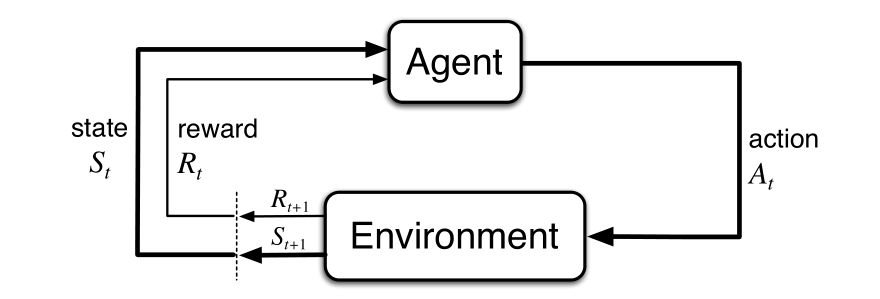
\includegraphics[scale=0.5]{rl-scheme}
\end{figure}

Формально, процесс взаимодействия агента и среды в обучении с подкреплением
таков:

\begin{itemize}
\item Задаются начальные \textit{стратегия агента} (\textit{англ.} policy)
  $\pi_1(a|s)$ и \textit{состояние среды} (\textit{англ.} state)
  $s_1 \in \mathcal{S}$
\item Для каждого момента времени $t = 1 \ldots T$:
  \begin{itemize}
  \item Агент выбирает \textit{действие} $a_t \in \mathcal{A}$ согласно
    вероятностному распределению, заданному текущей стратегией:
    $a_t ~ \pi_t(a | s_t)$;
  \item Агент получает от среды вознаграждение
    $r_{t+1} ~ p(r | a_t, s_t, r_t, a_{t-1}, s_{t-1}, \ldots, a_1, s_1)$ и
    среда переходит в новое состояние
    $s_{t+1} ~ p(s | a_t, s_t, r_t, a_{t-1}, s_{t-1}, \ldots, a_1, s_1)$;
  \item Агент корректирует стратегию $\pi_{t+1}(a | s)$.
  \end{itemize}
\end{itemize}

\begin{definition-ru}
  Модель взаимодействия агента и среды называется \textbf{марковским процессом
    принятия решений} (\textit{англ.} Markov decision process, MDP), если
  выполняется \textbf{марковское свойство}:
  вероятность получения вознаграждения $r'$ и перехода в состояние $s$ зависит
  только от текущего состояния и последнего действия:

  \begin{equation}
    P(r_{t+1} = r', s_{t+1} = s | a_t, s_t, r_t, a_{t-1}, s_{t-1}, \ldots, a_1,
    s_1) = P(r_{t+1} = r', s_{t+1} = s | a_t, s_t)
  \end{equation}
\end{definition-ru}

В большинстве случаев задача обучения с подкреплением формулируется именно как
марковский процесс принятия решений.

\begin{definition-ru}
  Стратегия агента $\pi(a | s)$ является \textbf{oптимальной}, если она
  максимизирует взвешенную сумму всех вознаграждений

  \begin{equation}\label{eq:reward-sum}
    \sum\limits_{t=0}^{\infty} {\gamma^t r_t} \,,
  \end{equation}

  где $0 \leqslant \gamma \leqslant 1$ --- \textit{коэффициент важности} для
  будущих выигрышей, для МППР без терминального состояния, или сумму

  \begin{equation}\label{eq:reward-sum}
    \sum\limits_{t=0}^{N} {r_t}
  \end{equation}

  для МППР с терминальным состоянием.
\end{definition-ru}

Во многих ситуациях, в число которых входят и случаи мультиагентных сред, агенту
недоступно полное состояние среды $s_t$, а только какая-то его часть. Для таких
случаев используется следующая модель:

\begin{definition-ru}
  \textbf{Частично наблюдаемый марковский процесс принятия решений}
  (\textit{англ.} Partially observed Markov decision process, POMDP) --- модель
  взаимодействия агента со средой, в котором вероятности вознаграждений и
  переходов между состояниями обладают марковским свойством, но стратегия агента
  $\pi(a | o)$ опирается на \textit{наблюдение} $o_t \in \mathcal{\Omega}$, а не
  на все состояние среды $s_t \in \mathcal{S}$. Наблюдение получается из
  состояния среды согласно заданному вероятностному распределению:
  $o_t ~ p(o | s_t)$
\end{definition-ru}

Существуют различные методы нахождения оптимальной стратегии для заданного MDP
или POMDP. В данной работе мы будем фокусироваться на методе \textit{Q-обучения}.

\begin{definition-ru}
  \textbf{Q-обучение} (\textit{англ.} Q-learning) \cite{q-learning-orig} ---
  метод нахождения оптимальной стратегии для MDP, заключающийся в построении
  функции ожидаемой полной стоимости
  $Q(s_{t'}, a_{t'}) \approx \sum\limits_{t=t'}^{\infty} \gamma^t r_t$. Текущее
  приближение $Q_{t+1}(s, a)$ обновляется при получении очередного
  вознаграждения $r_{t+1}$ за действие $a$ в состоянии $s$ и переходе в
  состояние $s'$ по формуле

  \begin{equation}\label{eq:q-learning}
    Q_{t+1}(s, a) = Q_t(s, a) + \alpha \left( r_{t+1} +
    \gamma \cdot \max\limits_{a \in \mathcal{A}} - Q_t(s', a) \right)
  \end{equation}

  Стратегия агента заключается в выборе действия с наибольшей ожидаемой полной
  стоимостью:

  \begin{equation}
    \pi_t(a | s) = \begin{cases}
      1, & a = \argmax\limits_{a \in \mathcal{A}} {Q_t(s, a)}\\
      0, & \text{otherwise}
    \end{cases}
  \end{equation}
\end{definition-ru}

В случае MDP с конечными множествами действий и состояний Q-обучение
гарантированно решает задачу обучения с подкреплением, т. е.
$Q_t(s, a) \xrightarrow{t \rightarrow \infty} Q^*(s, a)$ и $Q^*(s, a)$ порождает
оптимальную стратегию \cite{q-learning-orig}.

\section{Обзор методов обучения нейросетей с подкреплением}\label{overview:nns}

Первым громким успехом в области глубокого обучения с подкреплением стал
алгоритм Deep Q-Network (DQN) \cite{deepmind-dqn-orig}. Он основан на методе
Q-обучения, причем функция $Q(s, a)$ аппроксимируется нейронной сетью: на
входной слой подается значение текущего состояния $s$, на выходном слое
получаются значения $Q(s, a)$ для всех возможных $a \in \mathcal{A}$. 

В оригинальной работе агент учился играть в видеоигры для платформы Atari 2600.
Использовалась сверточная нейронная сеть, текущим состоянием $s$ являлось
изображение на экране и агент выбирал одно из возможных действий в игре.

Основной проблемой, с которой столкнулись авторы работы, стала неспособность
Q-обучения в чистом виде сойтись к оптимальному решению --- такая сходимость не
гарантируется для Марковских процессов с конечным числом состояний. Для борьбы с
этим эффектом в алгоритме DQN применено две эвристики: \textit{повторение опыта}
(\textit{англ.} experience replay) и \textit{целевая нейросеть} (\textit{англ.}
target network).

Повторение опыта заключается в сохранении всех встреченных эпизодов вида
$(s_t, a_t, r_t, s_{t+1})$ в массиве и осуществлении обновления Q-функции после
каждого действия не на основе этого действия и полученного за него
вознаграждения, а на основе случайной выборки из $k$ ранее встреченных эпизодов
($k$ --- параметр алгоритма). Таким образом, на каждом шаге обучения с некоторой
вероятностью учитывается весь опыт игры, а не только опыт последнего события,
что на практике приводит к стабилизации обучения.

Целевая нейросеть --- это подход, заключающийся в использовании отдельной
нейросети для вычисления опорных значений Q-функции при шаге Q-обучения. Веса из
обучаемой нейросети копируются в целевую только раз в $m$ шагов ($m$ ---
параметр алгоритма). Этот подход призван стабилизировать обучение путем
обеспечения одинаковых значений $Q(s_{t+1}, a)$ для одинаковых $s_{t+1}$ и $a$
на протяжении нескольких эпизодов.

В дальнейшем было изобретено множество модификаций оригинального алгоритма DQN.
Из них можно выделить модификацию с использованием приоритизированного
experience replay \cite{schaul2015prioritized}. Идея приоритизированного
experience replay заключается в том, чтобы с большей вероятностью доставать из
буфера эпизоды, сильнее всего повлиявшие на процесс обучения --- т. е. те,
где нейросеть ошибалась в своих оценках Q-функции сильнее всего.
Также были разработаны такие модификации алгоритма, как Double
DQN \cite{van2016deep}, основанный на идее двойного
Q-обучения \cite{hasselt2010double} и Dueling DQN \cite{wang2015dueling},
основанный на идее оценки Q-функции как отдельных величин --- ценности состояния
$V(s)$ и преимущества действия $A(a)$.

Также в работе \cite{hausknecht2015deep} было показано, что добавление
LSTM-слоя \cite{hochreiter1997long} в архитектуру нейросети позволяет добиться
лучших результатов при оптимизации частично наблюдаемых марковских процессов
благодаря сохранению информации о предыдущих наблюдениях в скрытом состоянии
рекуррентного слоя. В дальнейшем глубокие нейросети с рекуррентной архитектурой
показывали впечатляющие результаты в решении сложных задач, таких как игра
Doom \cite{lample2016playing}.

Одним из первых исследований по применению глубоких нейросетей в мультиагентной
среде является исследование \cite{tampuu2017multiagent}, в котором две нейросети
играли в игру Pong друг с другом. Но уже в работе \cite{foerster2016learning}
показано, что рекуррентные нейросети могут научиться пересылать друг другу сообщения для решения
совместных задач (в частности, в этом исследовании нейросети учились
разрабатывать совместную стратегию поведения для решения головоломки об узнике и
лампочке). На основе этой работы было проведено исследование
\cite{jorge2016learning}, в котором одна нейросеть обучалась
\enquote{задавать вопросы} другой, чтобы по полученным ответам угадать, какое из
изображений \enquote{загадала} другая нейросеть.

\section{DQN-routing}\label{overview:dqn-routing}

В бакалаврской выпускной квалификационной работе, выполненной автором данной
работы ранее, а также в статье \cite{mukhutdinov2019multi}, был
предложен алгоритм маршрутизации, объединениющий метода Q-routing с обучением
нейросетей --- \textit{DQN-routing}. Алгоритм был представлен как универсальный
алгоритм маршрутизации и протестирован в моделях компьютерной сети и конвейерной
системы. Эта секция посвящена краткому обзору на него.

\begin{algorithm}[!h]
\caption{Базовая логика алгоритма DQN-routing. $x$ -- метка текущего узла.}
\label{dqnr-pseudocode}
\begin{algorithmic}[1]
  \Function{Route}{$x$, $y$, $p$} \Comment{$y$ -- узел, пославший пакет, $p$ -- пакет}
    \State $s \gets $ \Call{GetState}{$x$, $p$}
    \State $\pi(a | s) \gets \textsc{Softmax}(Q_x(s, a))$ \Comment{Используем softmax-стратегию}
    \State $a \gets \pi(a | s)$
    \State $Q_e \gets \sum\limits_{a \in \mathcal{A}} {Q_x(s, a) \pi(a | s)}$
    \State $D_p^x \gets $ \Call{GetRewardData}{$s$, $p$}
    \State $S_x(p) \gets (s, a, D_p^x)$
    \State \Call{ReceiveReward}{$y$, $x$, $p$, $D_p^x$, $Q_e$}
    \State \Return $a$ \Comment{Возвращаем узел назначения}
  \EndFunction
  \Statex
  \Procedure{ReceiveReward}{$x$, $y$, $p$, $D_p^y$, $Q_e$}
    \State $(s, a, D_p^x) \gets S_x(p)$
    \State $r_a \gets $ \Call{ComputeReward}{$D_p^x$, $D_p^y$}
    \State $\Delta Q \gets r_a + Q_e - Q_x(s, a)$
    \State $Q_x(s, a) \approx Q_x(s, a) + \Delta Q$ \Comment{Шаг алгоритма оптимизации}
  \EndProcedure
\end{algorithmic}
\end{algorithm}

В листинге \ref{dqnr-pseudocode} приведена базовая логика алгоритма DQN-routing.
Сразу же заметно, что структура алгоритма очень похожа на Q-routing. Однако,
есть несколько ключевых отличий:

\begin{itemize}
\item Детали получения текущего состояния агента и порядок расчета
  вознаграждений абстрагированы;
\item Агент использует стохастическую стратегию, полученную применением функции
  softmax к текущим значениям Q-функции для доступных действий;
\item Соответственно, оценка дальнейшей стоимости пути пакета вычисляется как
  матожидание Q-функции относительно полученной стохастической стратегии;
\item Значение Q-функции обновляется не обычным сдвигом с некоторым learning
  rate, а с помощью алгоритма градиентной оптимизации (а именно, RMSProp \cite{tieleman2012lecture})
\end{itemize}

\begin{figure}[!h]
  \caption{DQN-routing: архитектура сети для графа из 5 узлов}\label{nn-pic-2}
  \centering
  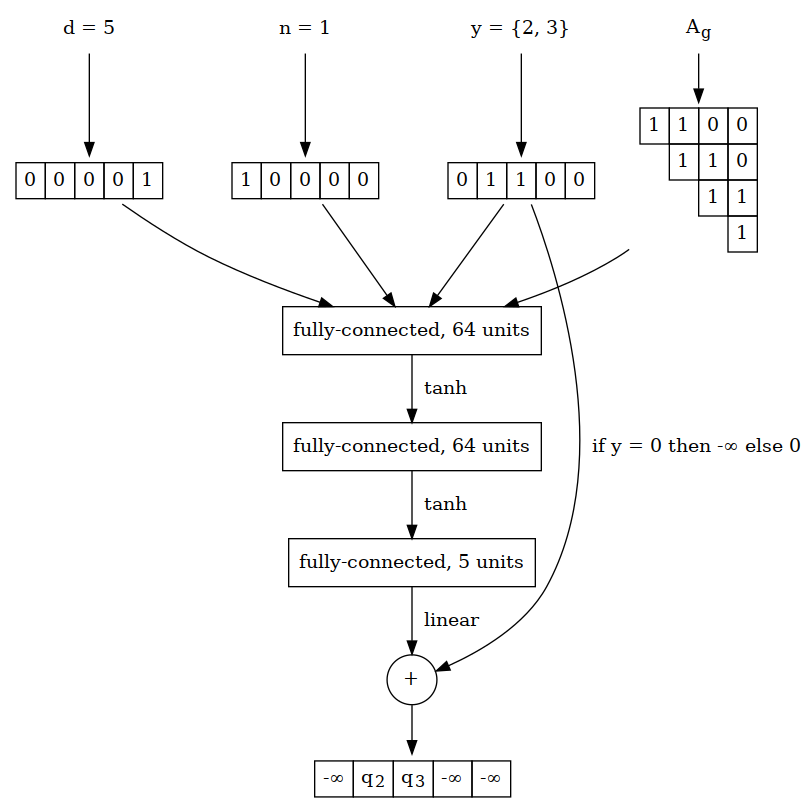
\includegraphics[scale=0.5]{nn-2}
\end{figure}

Функция $Q_x(s, a)$ в алгоритме DQN-routing аппроксимируется feed-forward
нейросетью с двумя скрытыми слоями по 64 нейрона. На вход
нейросети подается текущее состояние агента $s$, на выходе нейросети получаются
оценки $Q_x(s, a)$ для всех возможных действий $a$, где действие --- это узел, к
которому может быть перенаправлен пакет, причем если узел $u$
не является соседом $x$, то $Q_x(d, u) = -\infty$ (рис. \ref{nn-pic-2}).

\begin{algorithm}[!h]
\caption{Получение состояния агента в алгоритме DQN-routing}
\label{dqnr-pseudocode-getstate}
\begin{algorithmic}[1]
  \Function{GetState}{$x$, $p$}
    \State $d \gets dst(p)$ \Comment{Узел назначения пакета}
    \State $Y \gets \{ y | (x, y) \in E_x \}$ \Comment{Множество соседей}
    \State $A_x \gets $ \Call{AMatrix}{$G_x$} \Comment{Матрица смежности} 
    \State $X \gets $ \Call{AdditionalState}{$x$, $p$}
    \State \Return \Call{OneHot}{$x$} $\odot$ \Call{OneHot}{$d$} $\odot$
    \Call{OneHot}{$Y$} $\odot$ \Call{Flatten}{$A_x$} $\odot$ $X$
  \EndFunction
\end{algorithmic}
\end{algorithm}

Алгоритм также предусматривает поддержку каждым агентом модели сети в виде графа
с помощью протокола link-state (листинг \ref{ls-pseudocode}). Построение
текущего состояния агента приведено в листинге \ref{dqnr-pseudocode-getstate}.
Граф сети используется для включения в текущее состояние его матрицы смежности
наряду с метками текущего узла, узла назначения и множеством текущих соседних
узлов, закодированных унитарным кодом (\textit{англ.} one-hot encoding).

Реализация $\textsc{AdditionalState}$ зависит от области применения алгоритма: в
модели компьютерной сети эта функция возвращает пустой вектор, а в модели
конвейерной системы она возвращает вектор статусов соседних конвейеров (1 --
работает, 0 -- не работает) в том же унитарном коде.

Реализация функций $\textsc{GetRewardData}$ и $\textsc{ComputeReward}$ также
зависит от области применения:

\begin{itemize}
\item В модели компьютерной сети:
  \begin{itemize}
  \item $\textsc{GetRewardData}(s, p)$ = $\textsc{Time}()$;
  \item $\textsc{ComputeReward}(t_x, t_y)$ = $t_y - t_x$
  \end{itemize}
\item В модели конвейерной системы:
  \begin{itemize}
  \item $\textsc{GetRewardData}(s, p)$ = $(\textsc{Time}(), \textsc{EnergyGap}(x, p))$;
  \item $\textsc{ComputeReward}((t_x, \_), (t_y, e_p))$ = $(t_y - t_x) + \alpha e_p$
  \end{itemize}
\end{itemize}

То есть, в компьютерной сети вознаграждения аналогичны таковым в стандартном
Q-routing, а в конвейерной системе при расчете вознаграждения учитывается вклад
пересланного объекта в энергопотребление конвейера $\textsc{EnergyGap}(x, p)$.
Сам вклад рассчитывается как произведение постоянного энергопотребления
конвейера $k$ на неучтенное время работы: $e_p = p_k (t_y^k - t_e^k)$, причем
после каждого такого расчета текущее время работы считается учтенным:
$t_e^k \gets t_y^k$.

В бакалаврской работе и \cite{mukhutdinov2019multi} показано, что случайно
проинициализированные нейросетевые агенты с данной архитектурой при работе
онлайн не способны сойтись к оптимальной стратегии даже спустя долгое время,
вследствие фундаментальной нестационарности мультиагентной системы. Для борьбы с
этим предлагается использовать предварительное обучение с учителем, взяв за
опорные значения функции $Q_s(d, x)$ длину кратчайшего пути между $s$ и $d$,
проходящего через $x$.

Также было показано, что применение experience replay ухудшает
производительность предобученной модели в условиях изменяющегося трафика в сети.

\subsection{Недостатки DQN-routing}

Наиболе существенным недостатком DQN-routing является то, что размер нейросети
зависит от размера графа, в котором соответствующий агент работает как
маршрутизатор. Причем, если размер выходного слоя нейросети зависит от размера
графа линейно, то размер входного слоя зависит от него же квадратично, за счет
получения на вход графа в виде матрицы смежности.

Это накладывает существенные ограничения на применимость алгоритма сразу в
нескольких смыслах:

\begin{itemize}
\item Квадратичный рост входного слоя с ростом количества вершин в графе сильно
  ограничивает масштабируемость алгоритма, делая целесообразным его применение
  только в небольших графах до 100 вершин;
\item Предобученная модель с заданной архитектурой может работать только в
  графах с количеством вершин $n$, где $n$ --- размер выходного слоя модели;
\item Более того, необходимость предварительного обучения с учителем исключает
  свободный перенос модели на произвольный граф с $n$ вершин; возможна адаптация
  только к топологиям, не слишком сильно отличающихся от встреченных во время
  предварительного обучения. Фактически, модель неустойчива даже к
  перенумерованию вершин.
\end{itemize}

Почти все эти недостатки являются прямым следствием использования унитарного
кода при подаче номеров вершин на вход нейросети.

Помимо недостатков алгоритма самого по себе, также следует отметить, что для
проведения экспериментов в бакалаврской работе и \cite{mukhutdinov2019multi}
использовалась крайне упрощенная модель конвейерной системы. В этой модели не
отслеживались позиции отдельных объектов в системе, вместо этого их перемещение
и уровни загрузки конвейеров моделировались с помощью абстрактных понятий
\textit{текущего выходного потока}, \textit{текущего максимального потока} и
\textit{остаточного входного потока}, определенных для каждой из конвейерных
секций. Столкновения объектов не моделировались вовсе, т. е. подзадача избежания
столкновений в тех работах рассмотрена не была. Также, при моделировании
энергопотребления конвейеров было принято, что конвейеры потребляют постоянное
количество энергии за единицу времени, что, как было показано в разделе
\ref{overview:energy}, достаточно далеко от реальности.

Так как бакалаврская работа, в которой был предложен алгоритм DQN-routing, была
посвящена разработке обобщенного алгоритма маршрутизации, а не алгоритма
управления конвейерной системой, использование подобной далекой от реальности
модели конвейерной системы имело смысл --- оно позволяло продемонстрировать, что
алгоритм способен работать в системах, существенно отличающихся по поведению от
компьютерных сетей. Однако, подобная модель не подходит для честной оценки
работы алгоритма управления реальной конвейерной системой.

Таким образом, в настоящей работе можно выделить два ключевых направления:
\begin{itemize}
  \item Разработка приближенной к реальности имитационной модели конвейерной системы
  \item Разработка и тестирование алгоритма управления конвейерной системой,
    использующего идеи DQN-routing, но избавленного от его ключевых недостатков.
\end{itemize}

\chapterconclusion

В главе 1 была поставлена задача управления конвейерной системой. Задача была
разбита на подзадачи: маршрутизацию, избежание столкновений и оптимизацию
энергопотребления. Были рассмотрены существующие подходы к решению этих подзадач
применительно к конвейерным системам разных типов, их преимущества, недостатки и
границы применимости.

Также были рассмотрены существующие методы решения подзадачи маршрутизации
применительно к компьютерным сетям, их преимущества и недостатки.

Задача управления конвейерной системой была сформулирована в терминах обучения с
подкреплением; был намечен подход к ее решению. Также был проведен обзор
современных методов глубокого обучения с подкреплением, в том числе в
мультиагентной среде.

%% Так помечается конец обзора.
\finishrelatedwork

\chapter{Описание разработанного алгоритма}\label{chapter-algorithm}

\section{Архитектура системы и протокол взаимодействия между агентами}

В данной работе мы предполагаем децентрализованную архитектуру системы,
аналогичную той, что предложена в \cite{black2009intelligent,
  vyatkin-controllers} и частично описана в разделе \ref{vyatkin-method}. В
этой архитектуре реальными агентами, принимающими решения, являются контроллеры
отдельных конвейеров, управляющие собственной скоростью и поведением
отклонителей в своих сочленениях. Каждый контроллер соединен коммуникационным
интерфейсом только с контроллерами смежных конвейеров.

Каждое сочленение в системе будем представлять как узел графа, а конвейерные
секции между ними --- как ребра (рис. \ref{conveyor-graph-representation}).

\begin{figure}[!h]
  \caption{Пример представления конфигурации конвейерной системы в виде
    направленного графа}\label{conveyor-graph-representation}
  \centering
  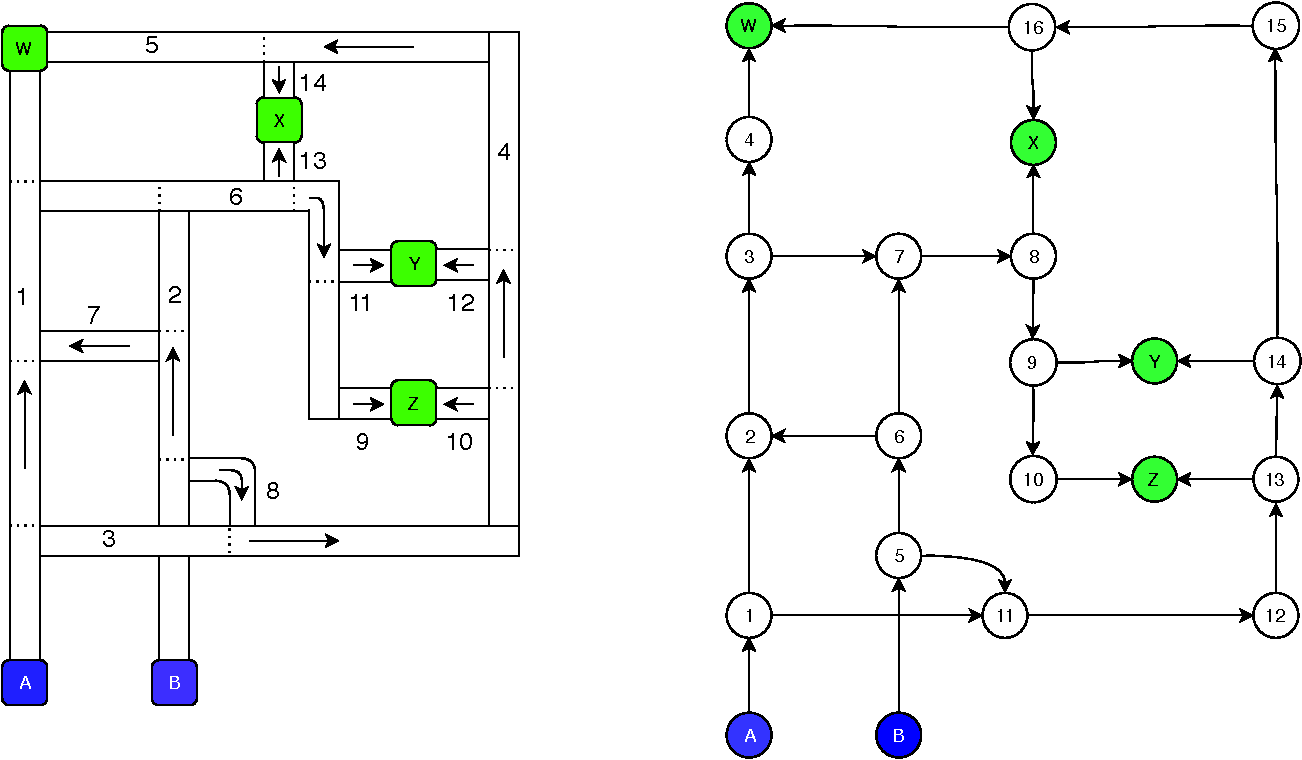
\includegraphics[width=\textwidth]{conveyor-1-illustration-2}
\end{figure}

Будем считать, что в каждом сочленении, в том числе в сходящихся сочленениях,
находится маршрутизирующий агент. Несмотря на то, что фиктивные маршрутизирующие
агенты, находящиеся в сходящихся сочленениях, не имеют выбора, куда послать
сумку, они нужны, чтобы в момент появления сумки в сочленении предсказывать
стоимость ее дальнейшего пути и посылать соответствующее сообщение с
вознаграждением агенту-отправителю сумки.

Предполагается, что каждому конвейеру известна собственная длина и длины
собственных секций. Конвейер поддерживает в памяти модель системы в виде графа,
где веса ребер равны длинам соответствующих секций конвейеров. Эта модель
формируется и обновляется с помощью link-state протокола.

Также предполагается, что конвейер может автоматически определять, что соседний
конвейер вышел из строя. В таком случае конвейер обновляет граф системы
соответствующим образом и распространяет это обновление с помощью link-state
протокола.

В отличие от работ \cite{black2009intelligent, vyatkin-controllers}, в этой
работе мы не уделяем внимания подробным техническим подробностям реализации
описанной логики в рамках определенного стандарта. Вместо этого мы фокусируемся
на высокоуровневой логике работы агентов. Для анализа работы предложенных
подходов разработана имитационная модель конвейерной системы при помощи языка
программирования Python и библиотеки дискретно-событийного моделирования Simpy.

\section{Формулировка задачи в терминах обучения с подкреплением}\label{rl-task-formulation}

В разделе \ref{problem-statement} задача управления конвейерной системой была
разбита на три подзадачи: маршрутизацию, избежание столкновений и
энергосбережение. Там же было указано, что недопустимость столкновений является
наиболее строгим ограничением в задаче, и был описан простой и надежный
существующий децентрализованный метод, гарантирующий отсутствие столкновений
\cite{black2009intelligent}. В связи с этим будем в нашем методе пытаться решать
только первую и третью подзадачи, и использовать его в комбинации с описанным
методом избежания столкновений для решения всей задачи целиком.

Задача маршрутизации заключается в минимизации среднего времени сумки в пути до
точки выгрузки:

\begin{equation}\label{eqs:J_r_avg}
  J'_R = \frac{1}{N} \sum\limits_{i=0}^{N} (t_d^i - t_s^i) \,,
\end{equation}

где $t_s^i$ --- время появления $i$-ой сумки в системе (сканирования), и
$t_d^i$ --- время ухода $i$-ой сумки в точку выгрузки, $N$ --- общее количество
сумок. Если общее количество сумок $N$ зафиксировано (а так как этот параметр не
является контролируемым, можем считать его зафиксированным), то с тем же успехом
можно минимизировать просто сумму времен сумок в пути:

\begin{equation}\label{eqs:J_r}
  J_R = \sum\limits_{i=0}^{N} (t_d^i - t_s^i) \,,
\end{equation}

Задача энергосбережения заключается в минимизации суммарного количества
потребленной энергии:

\begin{equation}\label{eqs:J_e}
  J_E = \int_0^T \! \sum\limits_{j=0}^{M} p_j(t) \; \mathrm{d}t \,,
\end{equation}

где $p_j(t)$ --- удельное энергопотребление конвейера $j$ в момент времени $t$,
$M$ --- количество конвейеров, $T$ --- полное время работы системы.

Соответственно, совместную задачу маршрутизации и энергосбережения можно
представить как минимизацию функции 

\begin{equation}
  J = \theta_R J_R + \theta_E J_E \,,
\end{equation}

где $\theta_R$ и $\theta_E$ --- это веса приоритета, параметры задачи.
Эквивалентно для удобства можно записать

\begin{equation}\label{eqs:J}
  J = J_R + \alpha J_E \,,
\end{equation}

где $\alpha = \frac{\theta_E}{\theta_R}$ --- приоритет оптимизации
энергопотребления.

Чтобы свести эту задачу к задаче обучения с подкреплением, то есть к задаче
поиска \textit{оптимальной стратегии}, нужно выразить $J$ в виде
(\ref{eq:reward-sum}). Чтобы это сделать, нам нужно определиться с тем, что в
системе является агентом, каково множество состояний агента $\mathcal{S}$,
каково множество действий $\mathcal{A}$ и как определена функция вознаграждения
$r : \mathcal{S} \times \mathcal{A}_s \rightarrow \Bbb{R}$.

Так как в наших целях разработка децентрализованного алгоритма, логично
предположить, что нужно рассматривать мультиагентный сеттинг, где в качестве
агента выступает контроллер отдельного конвейера, отвечающий за управление им и
отклонителями на его сочленениях, по аналогии с архитектурой, описанной в
разделе \ref{vyatkin-method}.

Если в этом случае рассматривать только функцию
энергопотребления $J_E$, и предположить, что конвейер $j$ может отслеживать
суммарное количество собственной потребленной энергии на момент времени $t$:

\begin{equation}
  P_j(t) = \int_0^t \! p_j(t) \; \mathrm{d}t \,,
\end{equation}

то достаточно взять в качестве действий изменение скорости и
включение/выключение питания, а в качестве состояний, скажем, текущую скорость и
количество сумок на конвейере. Тогда, выбрав некоторый период дискретизации
времени $\delta t$, мы можем определить функцию вознаграждения как
$r(s_t, a_t) = - (P_j(t + \delta t) - P_j(t))$. Тогда, взяв параметр
$\gamma = 1$, мы увидим, что формулы (\ref{eqs:J_e}) и (\ref{eq:reward-sum})
эквивалентны.

Подвох заключается в том, что в таком случае контроллер конвейера быстро
выяснит, что в любой ситуации ему не стоит двигаться, так как в разделе
\ref{overview:energy} было выяснено, что энергопотребление уменьшается с
уменьшением скорости. Такое поведение конфликтует с тем, что нам необходимо
все-таки доставлять сумки до точек назначения.

Можно предложить приоритизировать перемещение сумок над снижением
энергопотребления в рамках одного конвейера: конвейер двигается с максимально
возможной скоростью всегда, когда на нем находятся сумки, и останавливается
после того, как сумок на нем не осталось. То есть, мы оставляем конвейеру из
множества действий только действия ``on''/``off'', тем самым сводя задачу
оптимизации $J_E$ к задаче оптимального выключения.

Решение этой задачи в рамках одного конвейера элементарно и заключается в
выключении конвейера спустя определенный промежуток времени $d_t$ после того,
как его покинула последняя сумка. Задержка $d_t$ нужна потому что, во-первых,
конвейер не стартует и не запускается мгновенно, а имеет некоторые периоды
разгона и торможения, а во-вторых, потому что на разгон и торможение в
реальности уходит больше энергии, чем на равномерное движение за то же время.
Поэтому останавливаться моментально после того, как последняя сумка покинула
конвейер, неоптимально.

Если мы ограничим поведение агента таким образом, то, на первый взгляд, нам
останется решить только задачу маршрутизации --- отдельно минимизировать $J_R$.
Разобъем время сумки $i$ в пути от сканера к выгрузке $t_d^i - t_s^i$ на времена
пути по отдельным секциям конвейеров:
$t_d^i - t_s^i = \sum\limits_{j=0}^{n-1} (t_{j+1}^i - t_j^i)$, где $t_j^i$ ---
это время достижения сумкой $i$ $j$-го сочленения на пути, $t_0^i = t_s^i$,
$t_n^i = t_d^i$. Тогда, рассматривая в качестве действий отклонение или
пропускание сумки на сочленении с отклонителем, можно рассмотреть в качестве
вознаграждения время в пути, которое сумка проведет до следующего отклонителя.
Тогда, на первый взгляд, выражение для $J_R$ тоже совпадет с формулой
(\ref{eq:reward-sum}) и задачу можно будет считать решенной. Однако, это не
совсем так: это приведет к тому, что каждый отдельный конвейер будет вести себя
жадно --- всегда отклонять сумки вдоль самого быстрого пути до следующего
сочленения, потому что это будет максимизировать сумму вознаграждений, которые
получает именно он. Такая стратегия далеко не всегда будет приводить к тому, что
сумки будут отправляться по скорейшему пути до точки назначения.

Если же рассмотреть в качестве формального агента в системе не
конвейер, а \textit{сумку}, и рассмотреть ее текущую позицию в системе как часть
ее наблюдаемого состояния, то для такого агента минимизация суммы выигрышей
действительно будет приводить к движению по кратчайшему пути. Значит, для этого
агента можно (потенциально) найти оптимальную стратегию маршрутизации с помощью
Q-обучения.

Конечно, сумка не может физически реализовывать логику маршрутизации. Вместо
этого это делает контроллер конвеера, на котором она сейчас находится.
Заметим также, что путь сумки в системе конечен, а значит, конечно и
количество действий сумки-агента. Это значит, что параметр $\gamma$ в
(\ref{eq:q-learning}) можно взять равным 1. Тогда эта формула примет вид:

\begin{equation}
Q_x(o_t, a_t) = Q_x(o_t, a_t) + \alpha \left( r_t +
\gamma \cdot \max\limits_{a \in \mathcal{A}_{o_{t+1}}} Q_y(o_{t+1}, a) \right)
\end{equation}

Здесь $x$ и $y$ обозначают конвейеры, между которыми переместилась сумка ($x$
может совпадать с $y$),
а $r_t$ --- это вознаграждение, полученное ей за действие перенаправления (на
самом деле, контроллером конвейера, который совершил действие перенаправления, а
именно, $x$).

Если взять в качестве $r_t$ просто время в пути между сочленениями с минусом, то
максимизация суммы $r_t$ будет эквивалентна минимизации $J_R$. Если к тому же в качестве 
наблюдения сумки взять только идентификатор текущего сочленения, то получится в
точности алгоритм Q-routing.

Мы уже определились, что если ограничить доступные действия конвейерной
ленты как ``on''/``off'', то для оптимизации энергопотребления достаточно
простой стратегии остановки с задержкой после ухода сумок с конвейера.
Значит ли это, что использование алгоритма Q-routing в неизменном виде приведет
к оптимальной оптимизации энергопотребления в конвейерной системе? Нет, это не
так: прошлые рассуждения работали при условии, что агентом в системе считается
конвейер, а не сумка. Требуется модифицировать вознаграждения, чтобы учитывать
затраты на энергопотребление при маршрутизации. Если этого не сделать, то
оценки стоимостей путей сумок не будут никак учитывать энергопотребление, что
сделает невозможным, например, перенаправление сумок по более длинному пути
вдоль уже работающих конвейеров ради экономии энергии.

Будем рассчитывать полную стоимость пути сумки $i$ как

\begin{equation}
  C_i = (t_d^i - t_s^i) + \alpha e^i \,,
\end{equation}

где $t_s^i$ --- время появления сумки в источнике, $t_d^i$ --- время достижения
сумкой точки выгрузки, $\alpha$ --- это коэффициент важности энергосбережения
(параметр), а $e^i$ --- это энергетические затраты на перемещение чемодана,
порядок расчета которых нам предстоит определить. Суммарная стоимость всех
путей, таким образом, будет равна

\begin{equation}\label{eqs:J_c}
  J_c = \sum\limits_{i=0}^{N} C_i = \sum\limits_{i=0}^{N} (t_d^i - t_s^i)
  + \alpha \sum\limits_{i=0}^{N} e^i = J_R + \alpha \sum\limits_{i=0}^{N} e^i
\end{equation}

Заметим, что $J_c$ отличается от $J$ (уравнение (\ref{eqs:J})) только тем, что
вместо $J_E$ стоит сумма энергозатрат на перемещение всех сумок
$\sum\limits_{i=0}^{N} e^i$. То есть, если мы определим энергозатраты на
перемещение сумки $e^i$ таким образом, что сумма всех таких энергозатрат будет
отличаться от $J_E$ на константу, то минимизация $J_c$ будет эквивалентна
минимизации $J$.

Пусть $e^i$ считается как сумма энергозатрат на перемещение сумки вдоль каждой
конвейерной секции на пути сумки $i$:

\begin{equation}
  e^i = \sum\limits_{j \in path(i)} e_j^i
\end{equation}

Как определить $e_j^i$? Сделаем так, чтобы сумма всех энергозатрат
$\sum\limits_{i=0}^N e_j^i$ для всех секций $j$, принадлежащих конвейеру $k$,
отличалась от суммарных энергозатрат на работу этого конвейера на константу:

\begin{equation}\label{eqs:some-equality}
  \int_0^T \! p_k(t) \; \mathrm{d}t = \sum\limits_{j \in sections(k)} \sum\limits_{i=0}^N e_j^i + C
\end{equation}

Если мы сумеем этого добиться, то тогда $J_c$ и $J$ будут эквивалентны.
Определим $e_j^i$ так:

\begin{equation}
  e_j^i = \int_{t_k^e}^{t_j^i} \! p_k(t) \; \mathrm{d}t = P_k(t_j^i) -
  P_k(t_k^e) \,,
\end{equation}

где $t_j^i$ --- это время покидания сумкой $i$ секции $j$, а $t_k^e$ ---
это \textit{время последней регистрации} потраченной конвейером $k$
электроэнергии.

Поясним смысл величины $t_k^e$. Будем считать, что расчет $e_j^i$ производится в
тот же момент, что и расчет временных затрат на прохождение сумкой $i$ секции
$j$ --- то есть, в момент покидания сумкой этой секции. Если в момент $t_j^i$
покидания сумкой любой из секций конвейера мы будем регистрировать текущее
суммарное энергопотребление конвейера $P_k(t_j^i)$, то $e_j^i$ можно считать как

\begin{equation}
  e_j^i = P_k(t_j^i) - P_k^r \,,
\end{equation}

где $P_k^r$ --- это предыдущее зарегистрированное cуммарное энергопотребление
(т. е. значение $P_k^r$ обновляется каждый раз, когда сумка покидает одну из
секций конвейера $k$).

Таким образом, энергозатраты на перемещение сумки $i$ вдоль секции $j$
имеют смысл ``количество потраченной энергии, которое было учтено вследствие
проезда сумки по секции''. Энергозатраты на перемещение всех сумок по конвейеру
тогда составят

\begin{equation}
  P'_k = \sum\limits_{i=1}^{c_k} (P_k(t_i) - P(t_{i-1})) = P_k(t_{c_k}) -
  P_k(t_0) = P_k(t_{c_k}) \,,
\end{equation}

где $c_k$ --- количество всех событий пересечения сумкой какого-либо сочленения
конвейера $k$, $t_i$ --- время $i$-го такого события, $t_0 = 0$, $P_k(0) = 0$.

То есть, сумма определенных нами энергозатрат на прохождение сумок вдоль одного
конвейера оказывается равной суммарным энергозатратам этого конвейера на момент
времени $t_{c_k}$ ухода последней сумки с этого конвейера. Однако, конвейер
останавливается только через некоторое время $d_t$ после ухода с него последней
сумки, так что эта величина не равна полному количеству потребленной конвейером
энергии за все время. Однако, так как $d_t$ --- это константная величина, и так
как после $t_{c_k}$ на конвейере по определению не осталось сумок и он может
двигаться с максимально возможной скоростью, дополнительные энергозатраты на
этот финальный этап работы конвейера можно считать константными. Действительно,
как было рассмотрено в разделе \ref{overview:energy}, на энергопотребление
конвейера из переменных параметров влияют только свойства перемещаемого груза и
скорость конвейерной ленты. После $t_{c_k}$ свойства перемещаемого груза
постоянны (груза на ленте нет), и скорость может быть постоянной (максимальной).
Таким образом, энергию, потребленную конвейером после $t_{c_k}$ можно считать
константой, что приводит к тому, что тождество \ref{eqs:some-equality}
выполняется.

Итак, мы определили стоимости прохождения сумки вдоль секций конвейера таким
образом, чтобы минимизация суммарной стоимости всех путей сумок была
эквивалентна минимизации истинной целевой функции $J$. Тогда определим
вознаграждение за перенаправление сумки $i$ на секцию $j$ как

\begin{equation}
  r_j^i = -(t_j^i + \alpha e_j^i) \,,
\end{equation}

где $t_j^i$ --- время прохождения сумкой секции. При таких вознаграждениях
максимизация суммы вознаграждений (\ref{eq:reward-sum}) для агента-сумки
эквивалентно минимизации стоимости пути. Таким образом, используя принцип
Q-обучения для обучения агентов, мы будем минимизировать стоимость пути для
каждой сумки в отдельности. Это не строго эквивалентно минимизации суммарной
стоимости путей всех сумок $J_c$ (что, как было показано, эквивалентно
минимизации $J$), так как пути сумок пересекаются и действия одного агента
влияют на вознаграждения другого, но в большинстве случаев, в особенности в
отсутствие заторов на конвейерах, решениями этих двух задач являются одни и те
же (или очень похожие) стратегии.

\section{Алгоритм маршрутизации}

Так как в разделе \ref{rl-task-formulation} в процессе сведения задачи
управления конвейерной системой к задаче обучения с подкреплением получилось, по
сути, что все свелось к задаче маршрутизации, мы будем разрабатывать алгоритм в
два этапа:

\begin{enumerate}
\item Предложение нейросетевого алгоритма маршрутизации в абстрактной
  компьютерной сети, аналогичного Q-routing;
\item Проведение первичного экспериментального исследования алгоритма в модели
  абстрактной компьютерной сети;
\item Модификация предложенного алгоритма и вознаграждений для работы в
  конвейерной системе.
\end{enumerate}

Такой подход имеет следующие преимущества:

\begin{enumerate}
\item Маршрутизация в абстрактной компьютерной сети --- это почти подзадача
  маршрутизации в конвейерной сети в чистом виде, проще сначала решить подзадачу
\item Симуляция компьютерной сети существенно менее вычислительно затратна, что
  позволяет проще проводить эксперименты на начальном этапе исследования
\item Демонстрируется обобщаемость предложенного метода на более широкий класс
  задач
\end{enumerate}

\subsection{DQN-LE-routing}

Как было указано в разделе \ref{overview:dqn-routing}, корнем большинства проблем с алгоритмом
DQN-routing является использование унитарного кода для кодирования подаваемых на
вход нейросети вершин в графе. Номера вершин нельзя подавать на вход в чистом
виде, так как это неупорядоченные категориальные данные --- близость номеров 9 и
10 не имеет ничего общего с близостью вершин 9 и 10 в случайном графе, но
нейронная сеть устроена так, что близость значений на выходном слое коррелирует
с близостью значений на входном.

Унитарный код является универсальным методом для кодирования любых
категориальных данных, предотвращающим любые нежелательные корреляции. Однако,
не все корреляции являются нежелательными --- в случае вершин в графе, более близкие
по реберному расстоянию вершины имеет смысл кодировать более близкими
значениями.

Методы отображения вершин графа в векторные пространства с более низкими
размерностями называются \textit{графовыми эмбеддингами} (\textit{англ.} graph
embeddings). Существует множество алгоритмов для получения эмбеддингов из вершин
графа \cite{cai2018comprehensive, goyal2018graph}, различающихся по свойствам и
вычислительной сложности. 

Графовые эмбеддинги можно строить, основываясь на различных метриках похожести
вершин. Для целей усовершенствования алгоритма DQN-routing нам подойдут эмбеддинги,
сохраняющие информацию о локальной схожести вершин -- т. е. чем дальше друг от
друга находятся вершины, тем дальше друг от друга должны находиться вектора -- и
наоборот.

В целях получения эмбеддингов для подачи на вход нейросети в модифицированном
алгоритме DQN-routing был использован метод Laplacian Eigenmaps
\cite{belkin2002laplacian}. Метод заключается в следующем: при данной взвешенной
матрице смежности графа $W$ и заданной размерности эмбеддинга $k$ решается
обобщенная задача нахождения собственных векторов

\begin{equation}\label{eqs:lap}
  L y = \lambda D y \,,
\end{equation}

где $D$ - это диагональная матрица взвешенных степеней вершин графа,
$D_{ii}-\sum_j W_{ji}$, $L$ -- это матрица Кирхгофа для графа, $L = D - W$.

Если полученные собственные вектора $y_i$ отсортировать по возрастанию
соответствующих собственных чисел $\lambda_i$, то тогда результатом работы
алгоритма являются $k$ собственных векторов $y_1, ..., y_{k+1}$.
Эмбеддинг для $i$-го узла в сети можно получить как
$(y_1(i), ..., y_{k+1}(i))$.

Обозначим эту процедуру получения эмбеддингов из графа $G$ как $LE(G)$,
результатом процедуры будет матрица из собственных векторов $Y = LE(G)$
размерности $k \times n$, такая, что $i$-ый столбец матрицы $Y_i$ является
эмбеддингом для $i$-го узла.

Преимущества данного метода:
\begin{itemize}
\item Простота реализации
\item Скорость работы $O(|E|k^2)$ \cite{goyal2018graph} (при использовнии
  эффективной реализации разреженных матриц), что хорошо для разреженных графов
  --- а графы, представляющие конвейерные системы, достаточно разрежены;
\item Учет локальной схожести вершин --- близкие в графе вершины будут иметь
  близкие эмбеддинги, в то же время стоимости путей до близких вершин должны
  быть близки.
\item Линейность --- при одновременном сдвиге на некоторый вектор значения
  эмбеддингов не теряют смысла.
\end{itemize}

Данный метод работает только для ненаправленных графов, поэтому при
маршрутизации в направленных графах (как в конвейерных системах) будем строить
эмбеддинги по ним как по ненаправленным.

\begin{figure}[!h]
  \caption{DQN-LE-routing: архитектура сети}\label{nn-1-one-out}
  \centering
  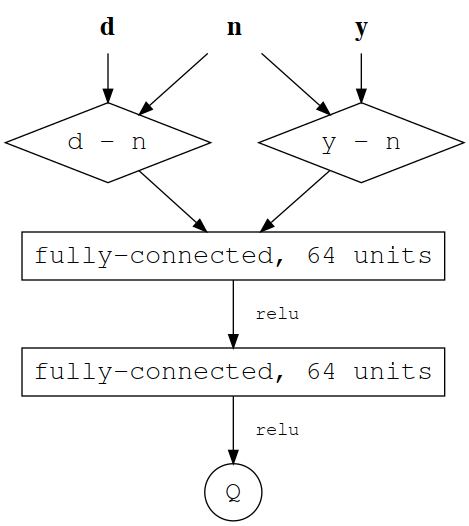
\includegraphics[scale=1]{nn-1-one-out}
\end{figure}

Кроме того, нам хочется, чтобы полученные эмбеддинги различались в графах,
отличающихся только весами ребер. Поэтому перед подсчетом $LE(G)$ будем находить
средний вес ребра $w'$ в $G$ и делить веса ребер на него. После получения
матрицы $Y$ будем домножать ее на $w'$, получая, таким образом, что в графе,
средняя длина ребер в котором в $\beta$ раз больше, чем в данном, среднее
расстояние между эмбеддингами будет также в $\beta$ раз больше.

Кодируя номера узлов эмбеддингами размерности $k$, мы только частично решаем
проблему зависимости размеров нейросети от количества узлов в графе. Выходной
слой все еще имеет размер $n$, и на вход все еще подается матрица смежности.

Первую проблему решим просто: откажемся от предсказания значений функции
$Q(s, a)$ сразу для нескольких действий (соседних узлов) $a$, и вместо этого
будем подавать конкретного соседа в виде эмбеддинга на входной слой.

Вторую проблему решим, просто отказавшись от подачи матрицы смежности на вход.
Она была необходима для того, чтобы адаптироваться к изменениям в топологии
сети. Однако, эмбеддинги уже содержат в себе информацию о топологии, поэтому при
ее изменении будем просто перестраивать $LE(G)$ на обновленном графе $G$.

Так как эмбеддинги линейны, каждый отдельный агент может считать, что он
находится в ``центре мира'' --- начале координат, а эмбеддинги остальных узлов
сдвинуты соответствующим образом. Таким образом, на вход нейросети достаточно
подать только два сдвинутых эмбеддинга, соответствующих узлу назначения и
соседу, для которого делается предсказание Q-функции.

Итого,
\begin{equation}
  Q_n(d, y) = f_{\theta}( (LE(G)_d - LE(G)_n) \odot (LE(G)_y - LE(G)_n)) \,,
\end{equation}

где $f_{\theta}$ --- это feed-forward нейросеть (рис. \ref{nn-1-one-out})

Эксперименты в модели абстрактной компьютерной сети (раздел
\ref{experiments:network}) показывают, что полученная модификация алгоритма,
которую мы назовем DQN-LE-routing, способна адаптироваться к изменениям
топологии и нагрузки не хуже оригинального DQN-routing, но при этом обученная
модель способна работать также и в ранее не встреченных графах, в том числе
графах большей размерности.

\chapterconclusion

В данной главе была описана модификация разработанного ранее алгоритма
DQN-routing --- DQN-LE-routing, избавленная от ключевых недостатков первого.
Также был предложен метод расчета вознаграждений для агентов в конвейерной сети,
позволяющий оптимизировать ее энергопотребление.

\chapter{Эксперименты}\label{experiments}

Экспериментальное сравнение разработанных алгоритмов проводилось в двух
имитационных моделях: модели абстрактной компьютерной сети и модели конвейерной
системы. Эксперименты в модели абстрактной компьютерной сети использовались для
того, чтобы проверять работоспособность базовой структуры рассматриваемого
алгоритма в относительно простом сеттинге. Кроме того, симуляция компьютерной
сети является менее вычислительно интенсивной задачей, чем симуляция конвейерной
системы. Также, существуют хорошо изученные способы генерации случайных графов,
обладающих топологическими свойствами, аналогичными таковым у реальных
компьютерных сетей (например, модель Барабаши-Альберт
\cite{albert2002statistical}), в то время как случайная генерация правдоподобных
моделей конвейерной сети является нетривиальной нерешенной задачей. Все это
делает модель компьютерной сети хорошей площадкой для первичного анализа
разработанного алгоритма.

Стоит, однако, подчеркнуть, что рассматривается модель \textit{абстрактной}
компьютерной сети. Отличие рассматриваемой модели от модели реальной
компьютерной сети заключается в том, что служебные сообщения передаются между
узлами мгновенно, в отличие от целевых пакетов, которые испытывают задержку при
проходе по соединениям и в очередях обработки на узлах. Это сделано для того,
чтобы приблизить модель абстрактной компьютерной сети к модели реальной
конвейерной сети.

Каждый тестовый сценарий для каждого типа алгоритма был запущен трижды с
различными числами инициализации генератора случайных чисел (были использованы
числа 42, 43 и 44). Целевые значения усреднялись на временных отрезках в 500
единиц времени модели. На представленных графиках линиями представлены значения,
усредненные по трем запускам сценария; соответствующими линиям полупрозрачными
полосами изображены разбросы между минимальным и максимальным значениями по трём
запускам.

\section{Эксперименты в модели абстрактной компьютерной сети}\label{experiments:network}

\begin{figure}[!h]
  \caption{Базовый граф для тестов в модели компьютерной сети}\label{fig-simple-network}
  \centering
  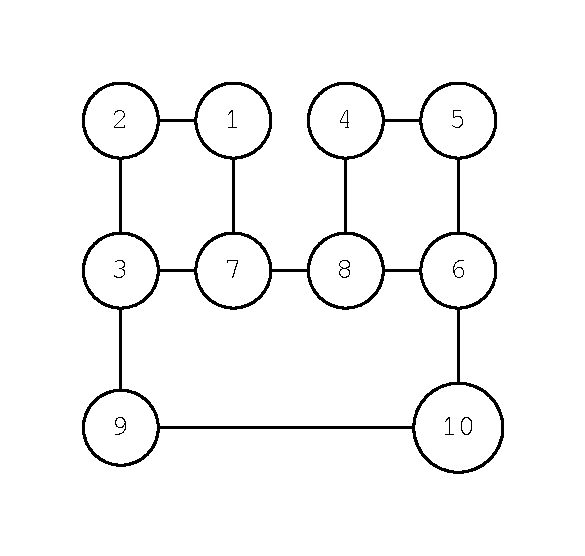
\includegraphics[scale=0.6]{graph-2.pdf}
\end{figure}

При проведении экспериментов в модели абстрактной компьютерной сети алгоритм
DQN-LE-routing сравнивалcя со следующими бейзлайнами:

\begin{itemize}
  \item \textbf{Shortest paths (SP)}: aлгоритм кратчайших путей с постоянными
    весами ребер использующий протокол link-state;
  \item \textbf{Q-routing}: алгоритм на основе табличного обучения с
    подкреплением, описанный в разделе \ref{q-routing-desc}, на идеях которого
    базируются алгоритмы DQN-routing и DQN-LE-routing;
  \item \textbf{DQN-routing}: алгоритм, ранее предложенный автором данной
    работы, рассмотренный в разделе \ref{overview:dqn-routing}.
\end{itemize}

Нейросетевые агенты для алгоритмов DQN-routing и DQN-LE-routing перед работой
проходили предварительное обучение с учителем на эпизодах работы алгоритма
кратчайших путей внутри графа из 10 вершин (Рис.~\ref{fig-simple-network}).
Каждое соединение в графе имеет задержку 10 мс и пропускную способность 1024 байт/мс.
Каждый пакет имеет размер 1024 байт, каждый роутер обрабатывает один пакет за 5
мс. Алгоритм кратчайших путей в качестве веса ребра использует его задержку.

Всего было сгенерировано 230000 эпизодов, включая эпизоды работы на версиях
данного графа с некоторыми отсутствующими ребрами. Для DQN-LE агента
использовались графовые эмбеддинги размерности 8. Оба нейросетевых агента
обучались на данных в течение 10 эпох с помощью алгоритма RMSProp \cite{tieleman2012lecture}.

\subsection{Адаптация к изменению нагрузки на сеть}

\begin{figure}[!h]
  \caption{Резкое понижение и последующее снижение нагрузки}\label{experiments:network:peak-load-small}
  \centering
  \includegraphics[width=\textwidth]{peak-load-small}
\end{figure}

В этом сценарии пакеты перемещаются между двумя половинами
графа \ref{fig-simple-network} (между множествами вершин $\{1, 2, 3, 7\}$ и
$\{4, 5, 6, 8\}$). Сначала пакеты посылаются раз в 10 мс, затем нагрузка резко
возрастает --- пакеты посылаются с периодом 3.5 мс ---, и в конце падает вновь.

При резком повыщении нагрузки роутеров статический link-state алгоритм не
способен работать эффективно, как видно на графике
\ref{experiments:network:peak-load-small}, так как очереди маршрутизаторов,
через которых проходит большинство кратчайших путей между половинами сети
(узлы 7 и 8 на рис. \ref{fig-simple-network}), начинают переполняться, и
пакеты начинают застревать в этих очередях, вызывая стремительный рост среднего
времени на доставку. Все прочие алгоритмы оказываются способны быстро обнаружить
затор и направить трафик по обходному пути.

\subsection{Адаптация к обрывам и восстановлениям соединений}\label{experiments:simple/links}

\begin{figure}[!h]
  \caption{Обрыв и последующее восстановление трех соединений}\label{experiments:network:topology-change-small}
  \centering
  \includegraphics[width=\textwidth]{topology-change-small}
\end{figure}

В этом сценарии при небольшой нагрузке в сети производился последовательный
обрыв соединений $(7, 8)$, $(1, 2)$ и $(5, 6)$ и последующее их восстановление в том
же порядке. Пакеты посылались, как и в предыдущем сценарии, между двумя
половинами графа \ref{fig-simple-network}.

Как видно на графике \ref{experiments:network:topology-change-small}, алгоритмы
DQN- и DQN-LE-routing в этом сценарии работают почти в точности так же, как и
оптимальный в этой ситуации алгоритм кратчайших путей, в то время как Q-routing
не способен вернуться к оптимальному поведению после восстановления всех
соединений. При этом DQN-LE-routing обеспечивает такое поведение без
использования подачи матрицы смежности графа на вход нейросетевого агента,
только за счет перестроения эмбеддингов при изменении топологии сети.

\subsection{Перенос опыта на новые топологии графов}

Необходимость предобучения для работы в графе заданной топологии является
существенным недостатком алгоритма DQN-routing, сильно ограничивающим его
практическую ценность. Алгоритм DQN-LE-routing тоже требует предобучения, но
благодаря использованию графовых эмбеддингов обобщающая способность единожды
обученной модели гораздо выше.

\begin{figure}[!h]
  \caption{Случайный граф из 10 вершин}\label{fig-random-net-10n}
  \centering
  \includegraphics[scale=0.7]{random-graph-10n}
\end{figure}

Нейросетевые агенты для алгоритмов DQN- и DQN-LE-routing, обученные на данных с
базового графа из 10 вершин (рис. \ref{fig-simple-network}), были использованы
для работы в случайном графе из 10 вершин, сгенерированном по модели
Барабаши-Альберт с параметром $m = 2$ и случайными значениями задержки
соединений от 10 до 20 мс. Прочие параметры сгенерированного графа идентичны
таковым в базовом графе. 

\begin{figure}[!h]
  \caption{Перенос опыта на новую топологию графа}\label{experiments:network:transfer-small}
  \centering
  \includegraphics[width=\textwidth]{learning-transfer-small}
\end{figure}

График \ref{experiments:network:transfer-small} демонстрирует показатели работы
алгоритмов в новом графе при низкой нагрузке. Работа алгоритма кратчайших
путей (оптимального при низкой нагрузке) также приведена для сравнения. Видно,
что DQN-routing ведет себя в новом графе хаотично и даже не способен сойтись к
какой-либо стабильной стратегии. В отличие от него, DQN-LE-routing работает
оптимально (аналогично алгоритму кратчайших путей) с самого начала, что
позволяет сделать вывод, что опыт нейросети, полученый при обучении, очень
хорошо обобщается на графы того же размера.

\begin{figure}[!h]
  \caption{Случайный граф из 40 вершин}\label{fig-random-net-40n}
  \centering
  \includegraphics[scale=0.7]{random-graph-40n}
\end{figure}

\begin{figure*}[!h]
  \centering
  \subfloat[Низкая нагрузка]{
    \includegraphics[width=0.4\textwidth]{learning-transfer-big-low-load}
    \label{experiments:network:transfer-big-low}}
  \hfil
  \subfloat[Высокая нагрузка]{
    \includegraphics[width=0.4\textwidth]{learning-transfer-big-high-load}
    \label{experiments:network:transfer-big-high}}
  \caption{Перенос опыта на новую топологию большего размера}\label{experiments:network:transfer-big}
\end{figure*}

Нейросетевой агент алгоритма DQN-routing, обученный на графе с $N$ вершинами,
принципиально не может работать на графах большего размера, однако
DQN-LE-routing свободен от этого ограничения, так как векторные представления
заданной размерности $d$ можно получить для вершин любого графа. На графиках
\ref{experiments:network:transfer-big-low} и
\ref{experiments:network:transfer-big-high} изображена работа алгоритма
DQN-LE-routing, предобученного на базовом графе из 10 вершин, внутри случайного
графа из 40 вершин (рис. \ref{fig-random-net-40n}), в условиях низкой и высокой
нагрузки. В условиях низкой нагрузки DQN-LE-routing начинает показывать
приемлемое качество работы существенно быстрее, чем Q-routing, хоть и не
сходится к оптимальной стратегии аналогичной алгоритму кратчайших путей --- но к
ней не может сойтись и Q-routing. В условиях высокой нагрузки DQN-LE-routing
ведет себя существенно лучше обоих бейзлайнов --- shortest path переполняет
очереди ключевых узлов и расходится, Q-routing долгое время ведет себя хаотично,
прежде чем сойтись к очень неоптимальной стратегии, в то время как
DQN-LE-routing работает как часы.

Из результатов экспериментов можно сделать вывод, что предобученный DQN-LE-routing обладает
хорошей обобщающей способностью и способен успешно работать на большом множестве
различных графов.

\section{Эксперименты в модели конвейерной системы}\label{experiments:conveyors}

\begin{figure}[!h]
  \caption{Модель конвейерной системы для тестов}\label{test-conveyors}
  \centering
  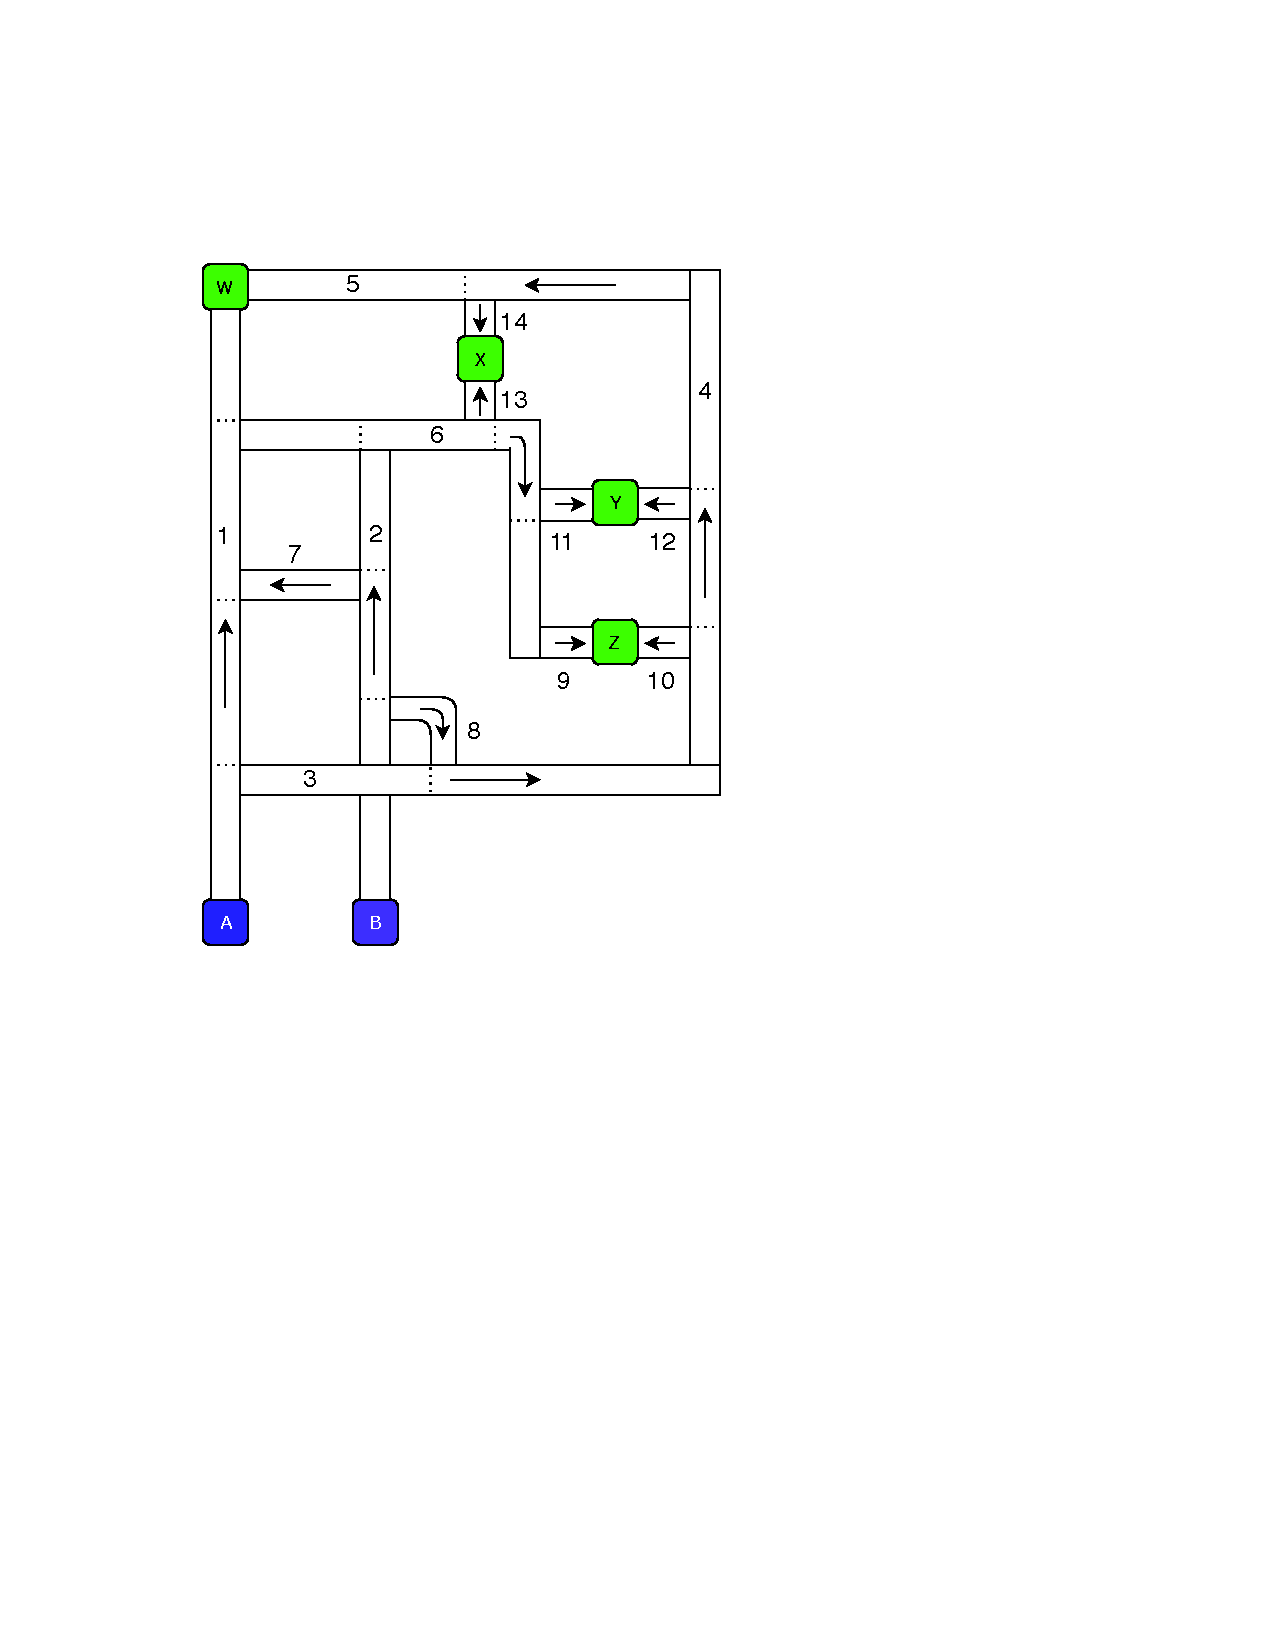
\includegraphics[width=0.4\textwidth]{conveyor-1-illustration-1}
\end{figure}

В отличие от модели компьютерной сети, в модели конвейерной системы алгоритм
будет пытаться оптимизировать не только среднее время доставки пакета
(чемодана), но и \textit{энергопотребление} конвейеров. Оптимизация
энергопотребления заключается в том, чтобы использовать для доставки чемоданов
до точек назначения как можно меньше конвейеров.

В алгоритме DQN-routing на вход нейросети будет дополнительно подаваться вектор
$w$ размера $n$ (где $n$ --- количество конвейерных секций в системе), в котором на $i$-ой
позиции стоит 0, если конвейер, на котором находится секция $i$, в данный момент
находится в состоянии ожидания, и 1 --- если он работает.

В алгоритме DQN-LE-routing при расчете Q-функции для соседней секции $x$ на вход
нейросети будет дополнительно подаваться число 1, если конвейер, на котором
находится секция $x$, работает, и 0 --- если не работает.

Эксперименты проводились на модели конвейерной сети из 14 конвейеров с 27
секциями в сумме, двумя входными вершинами и четырьмя выходными вершинами (рис.
\ref{test-conveyors}). Секции с первой по 20 имеют длину 10 метров, с 21 по 27 --- 2
метра. Энергопотребление каждого конвейера равно 1 кВт, максимальная
скорость --- 1 м/c.

\subsection{Неравномерный поток до выходных вершин}

Как можно видеть на иллюстрации \ref{test-conveyors}, кратчайший путь от входов
до выходов W и X пролегает через конвейеры 1, 2, 7 и 6, а до выходов Y и Z --
через конвейеры 1, 2, 3 и 4. Однако до выходов Y и Z также можно попасть через
конвейер 6, не задействуя конвейеры 3 и 4. Если для нас важно оптимизировать
энергозатраты, то в условиях небольшого входящего потока чемоданов такая
стратегия является более предпочтительной.

\begin{figure*}[!h]
  \centering
  \subfloat[Время сумок в пути]{
    \includegraphics[width=0.48\textwidth]{conveyors-new-1-time}
    \label{experiments:conveyors:1-time}}
  \hfil
  \subfloat[Энергопотребление системы]{
    \includegraphics[width=0.48\textwidth]{conveyors-new-1-energy}
    \label{experiments:conveyors:1-energy}}
  \caption{Неравномерный поток до выходных вершин}\label{experiments:conveyors:1}
\end{figure*}

В данном сценарии поток чемоданов попеременно идет либо только в выходы W и X,
либо во все четыре выхода сразу. Параметр важности экономии энергопотребления
$\alpha$ равен 1.

На иллюстрации \ref{experiments:conveyors:1} видно, что алгоритм DQN-LE-routing
после непродолжительного периода адаптации начинает работать
заметно лучше алгоритмов shortest paths и Q-routing с точки зрения экономии энергии,
жертвуя средним временем доставки чемодана. 

%% \subsection{Плавное повышение нагрузки}

%% \begin{figure*}[!h]
%%   \centering
%%   \subfloat[Время сумок в пути]{
%%     \includegraphics[width=0.4\textwidth]{conveyors2-late-time}
%%     \label{experiments:conveyors:2-late-time}}
%%   \hfil
%%   \subfloat[Энергопотребление системы]{
%%     \includegraphics[width=0.4\textwidth]{conveyors2-late-energy}
%%     \label{experiments:conveyors:2-late-energy}}
%%   \caption{Плавное повышение нагрузки: $\alpha = 1$, $\alpha_{LE} = 0.4$}\label{experiments:conveyors:2-late}
%% \end{figure*}

%% Первая половина этого сценария повторяет предыдущий --- поток попеременно идет то
%% во все выходы, то только в выходы W и X. Во второй половине сценария частота
%% появления чемоданов на входах возрастает в два раза и продолжает плавно расти.

%% В этом сценарии алгоритмы DQN- и DQN-LE-routing используют разные параметры
%% важности экономии энергопотребления, обоначенные соотв. $\alpha$ и
%% $\alpha_{LE}$, так как на практике алгоритм DQN-LE-routing оказался более
%% чувствительным к величине этого параметра.

%% \begin{figure*}[!h]
%%   \centering
%%   \subfloat[Время сумок в пути]{
%%     \includegraphics[width=0.4\textwidth]{conveyors2-early-time}
%%     \label{experiments:conveyors:2-early-time}}
%%   \hfil
%%   \subfloat[Энергопотребление системы]{
%%     \includegraphics[width=0.4\textwidth]{conveyors2-early-energy}
%%     \label{experiments:conveyors:2-early-energy}}
%%   \caption{Плавное повышение нагрузки: $\alpha = 0.8$, $\alpha_{LE} = 0.2$}\label{experiments:conveyors:2-early}
%% \end{figure*}

%% Графики \ref{experiments:conveyors:2-late}
%% и \ref{experiments:conveyors:2-early} показывают, что при постепенном
%% увеличении интенсивности трафика (и, как следствие, загруженности конвейеров)
%% алгоритмы DQN- и DQN-routing в какой-то момент начинают использовать конвейеры 3
%% и 4, чтобы снизить среднюю скорость доставки чемоданов, причем это происходит
%% тем раньше, чем ниже параметр $\alpha$ ($\alpha_{LE}$).

\chapterconclusion

Экспериментальное исследование показало, что алгоритм DQN-LE-routing, в отличие
от DQN-routing, способен адаптироваться к новым топологиям графов. Также были
проведены эксперименты в модели конвейерной сети, показывающие, что он способен
оптимизировать ее энергопотребление.

%% Макрос для заключения. Совместим со старым стилевиком.
\startconclusionpage

В данной работе был представлен новый метод управления конвейерной системой,
основанный на маршрутизации с помощью самообучающихся нейросетевых агентов ---
DQN-LE-routing. Для анализа работы алгоритма и его сравнения с существующими
аналогами была разработана имитационная модель штучной конвейерной сети.

В ходе экспериментального исследования было установлено, что, в отличие от
существующих аналогов, алгоритм способен успешно решать задачу совместной
оптимизации энергопотребления и времени доставки объектов. Также было показано,
что DQN-LE-routing превосходит по качеству работы предложенный ранее автором
алгоритм DQN-routing и обладает большим потенциалом применения в реальных системах.

%% Обратите внимание на heading. Без него тоже работает, но название будет другим.
\printmainbibliography

%% После этой команды chapter будет генерировать приложения, нумерованные русскими буквами.
%% \startappendices из старого стилевика будет делать то же самое
%% \appendix

%% \chapter{Промежуточные результаты исследования}\label{apx:bad-results}

%% TBD

%% Наиболее приближенная к реальности модель энергопотребления конвейера из
%% известных автору \cite{zhang2011modeling}, к сожалению, предназначена для расчета энергопотребления
%% конвейера для насыпных грузов.
%% Согласно , 

\end{document}
